\chapter{Teoretická část studentské práce}

\section{Přehled optického vlákna a jeho vlastností}

\subsection{Definice optického vlákna}

	Optické vlákno je válečkový dielektrický vlnovod, ve kterém se šíří elektromagnetické vlny (zpravidla světlo či infračervené záření) ve směru osy vlákna s využitím principu totálního odrazu na rozhraní dvou prostředí s rozdílným indexem lomu. Vnitřní část vlákna se nazývá jádro, okolo jádra je plášť a primární ochrana. K vazbě optického signálu na jádro musí být index lomu jádra vyšší, než má plášť. U optických vláken používaných v datových sítích se udává průměr jádra a pláště v mikrometrech, a používají se vlákna o průměrech 50/125 μm (standardizováno ITU-T podle G.651) nebo 62,5/125 μm (používá se především v USA). Průměr jádra vlákna od různých výrobců se však liší. To je ovlivněno typem vlákna, normami přijatými konkrétním výrobcem nebo státem \cite{3}. 

	Speciální kabely jsou vyráběny na bázi skleněných vláken, které se používají k realizaci optických komunikací na velké vzdálenosti. Současně je rychlost přenosu dat několikrát vyšší než v konvenční kabelové komunikací. Optické vlákno se také používá při výrobě různých senzorů \cite{3}.
	
\begin{figure}[h]
	\centering
	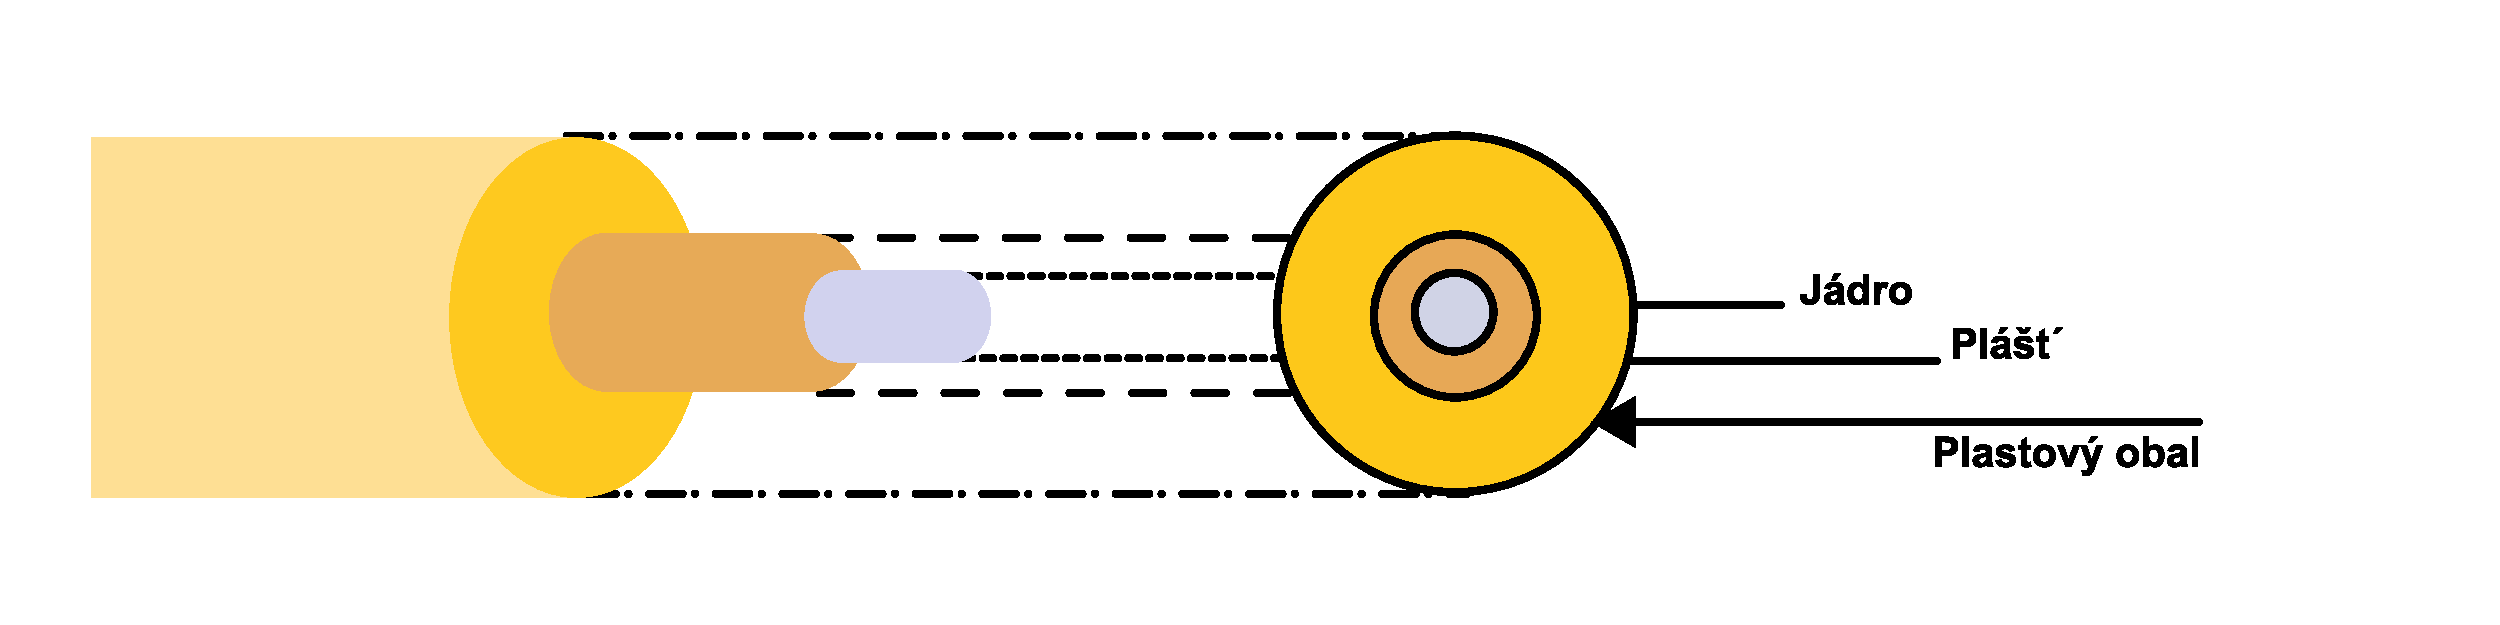
\includegraphics[width=13cm]{obrazky/02}
	\caption{Struktura optického vlákna\cite{3}}
	\label{fig:02}
\end{figure}

	Při výrobě optického vlákna se většinou používá křemenné sklo. Existují však různé modifikace vláken, například pro přenos infračervených signálů pomocí vlákna vyrobeného z fluorohlinitanu, fluoro-zirkoničitého nebo chalkogenidového skla. V moderním světě se skleněná optická vlákna postupně nahrazují plasty \cite{3}.

\subsection{Princip činnosti optického vlákna}

Optické vlákno používá základní vlastnosti geometrické optiky pro svou funkčnost. Princip činnosti optického vedení není složitý: světelným zdrojem přenášeným optickými kabely je LED (nebo polovodičový laser) a informace je kódována dvouúrovňovou změnou intenzity světla. Na druhém konci kabelu přijímací detektor převádí světelné signály na elektrické signály. Pro přenos na větší vzdálenost na okraji optického kabelu je umístěno speciální zařízení - zesilovač, který zvětšuje vzdálenost přenosu. Při spojování optických vláken se používají optické spojky, ve kterých jsou vlákna svařována dohromady \cite{3}.

	Pro přenos informací je nutné nejen vytvořit světelnou vlnu, ale také ji uložit a nasměrovat správným směrem. V homogenním prostředí se světlo šíří přímočaře, ale na hranici změny hustoty prostředí podle optických zákonů dochází ke změně směru (odrazu nebo lomu) \cite{3}.

	V aktuálně používaných obvodech je paprsek z LED nebo laseru propuštěn do hustšího prostředí omezeného méně hustým. Při správném výběru materiálů dochází k úplnému odrazu (refrakce chybí). Přenášený signál tedy <<jde>> uvnitř uzavřeného prostředí a vytváří cestu od zdroje signálu k jeho přijímači \cite{3}. 
	
\begin{figure}[h]
	\centering
	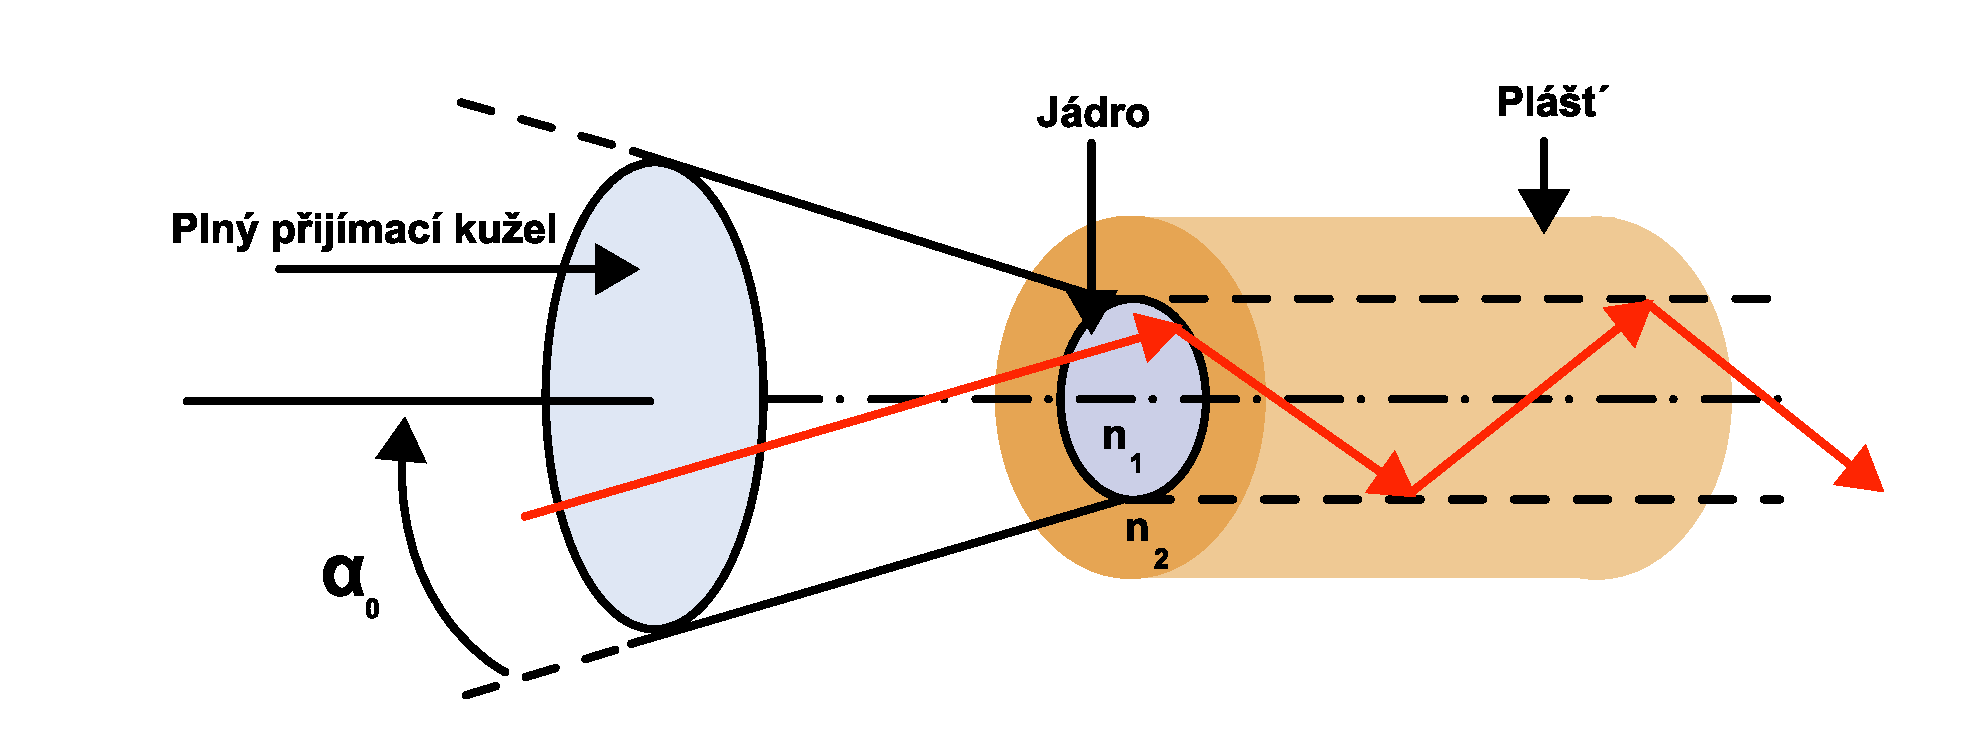
\includegraphics[width=13cm]{obrazky/03}
	\caption{Vstup světla do optického vlákna\cite{3}}
	\label{fig:03}
\end{figure}
	
	Paprsek světla se zavádí do vlákna pod malým úhlem $\alpha$. Schopnost vlákna přijímat světlo do jádra (maximální přijatelný úhel) je určena jeho numerickou aperturou~($NA$)\cite{3}.
	
\begin{equation}
NA = sin(\alpha_0) = \sqrt{n^2_1 - n^2_2},
\end{equation}
	
kde $\alpha_0$ je maximální vstupní úhel (tj. omezující úhel mezi osou a úhlem celkového odrazu jádra), $n_1$ je index lomu jádra a $n_2$ je index lomu pláště. Celkový přijímací kužel optického vlákna je definován jako $2\alpha_0$ \cite{3}.

\begin{figure}[ht]
	\centering
	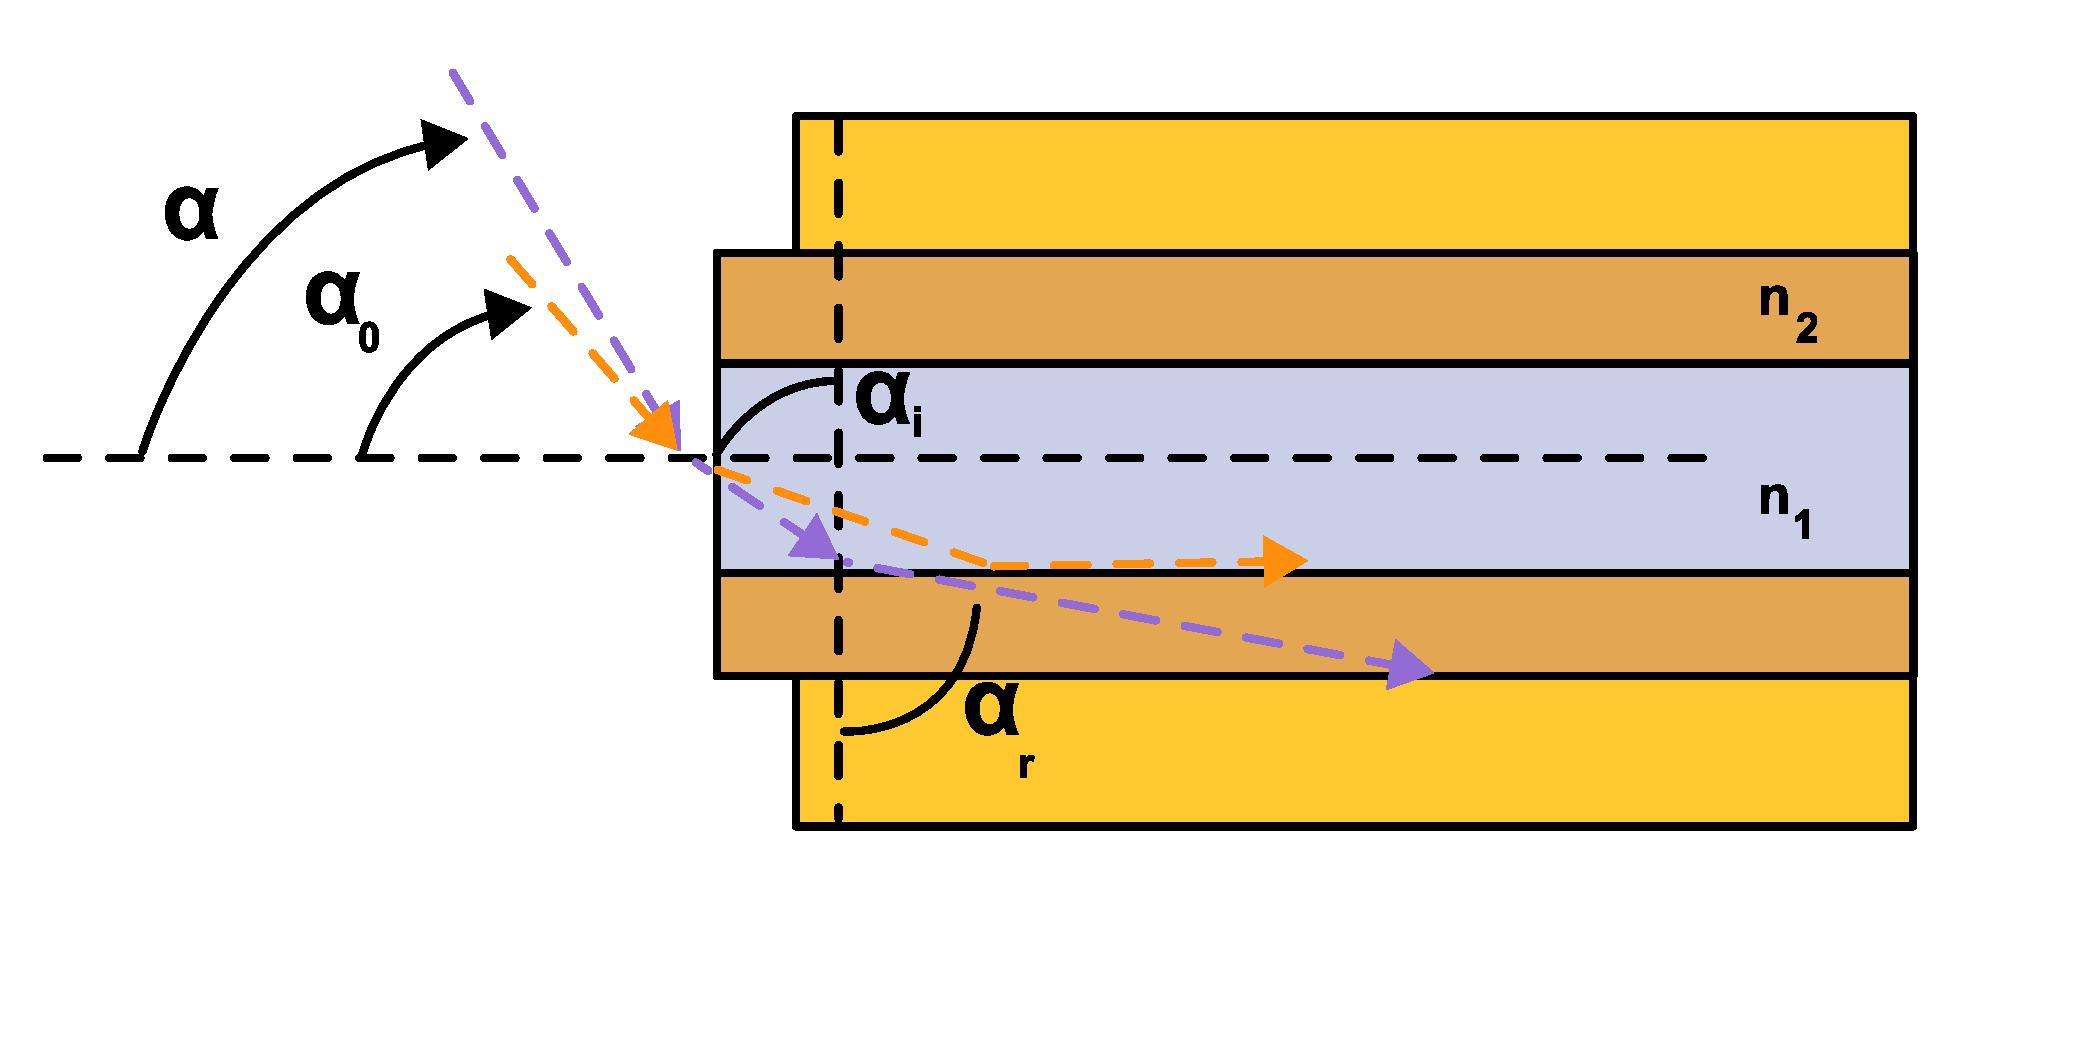
\includegraphics[width=9cm]{obrazky/09}
	\caption{Lom světla\cite{3}}
	\label{fig:09}
\end{figure}

Světelný paprsek se šíří v optickém vlákně podle Snell-Descartesova zákona. Část světla je přiváděna přes plný přijímací kužel optického vlákna. Fenomén lomu je vyjádřen změnou úhlu průchodu paprsku světla přes hranici dvou prostředí. Pokud $\alpha > \alpha_0$, paprsek je úplně lomený a opouští jádro \cite{3}.

\begin{equation}
n_1 sin(\alpha_i) = n_2 sin(\alpha_r)
\end{equation}

Odrážení je změna směru světelného paprsku na hranici mezi dvěma prostředími. V tomto případě se světelný paprsek vrací do jádra, ze kterého pochází.
Když $\alpha < \alpha_0$, paprsek se odráží a zůstává v jádru \cite{3}.

\begin{equation}
\alpha_i = \alpha_r.
\end{equation}

\begin{figure}[ht]
	\centering
	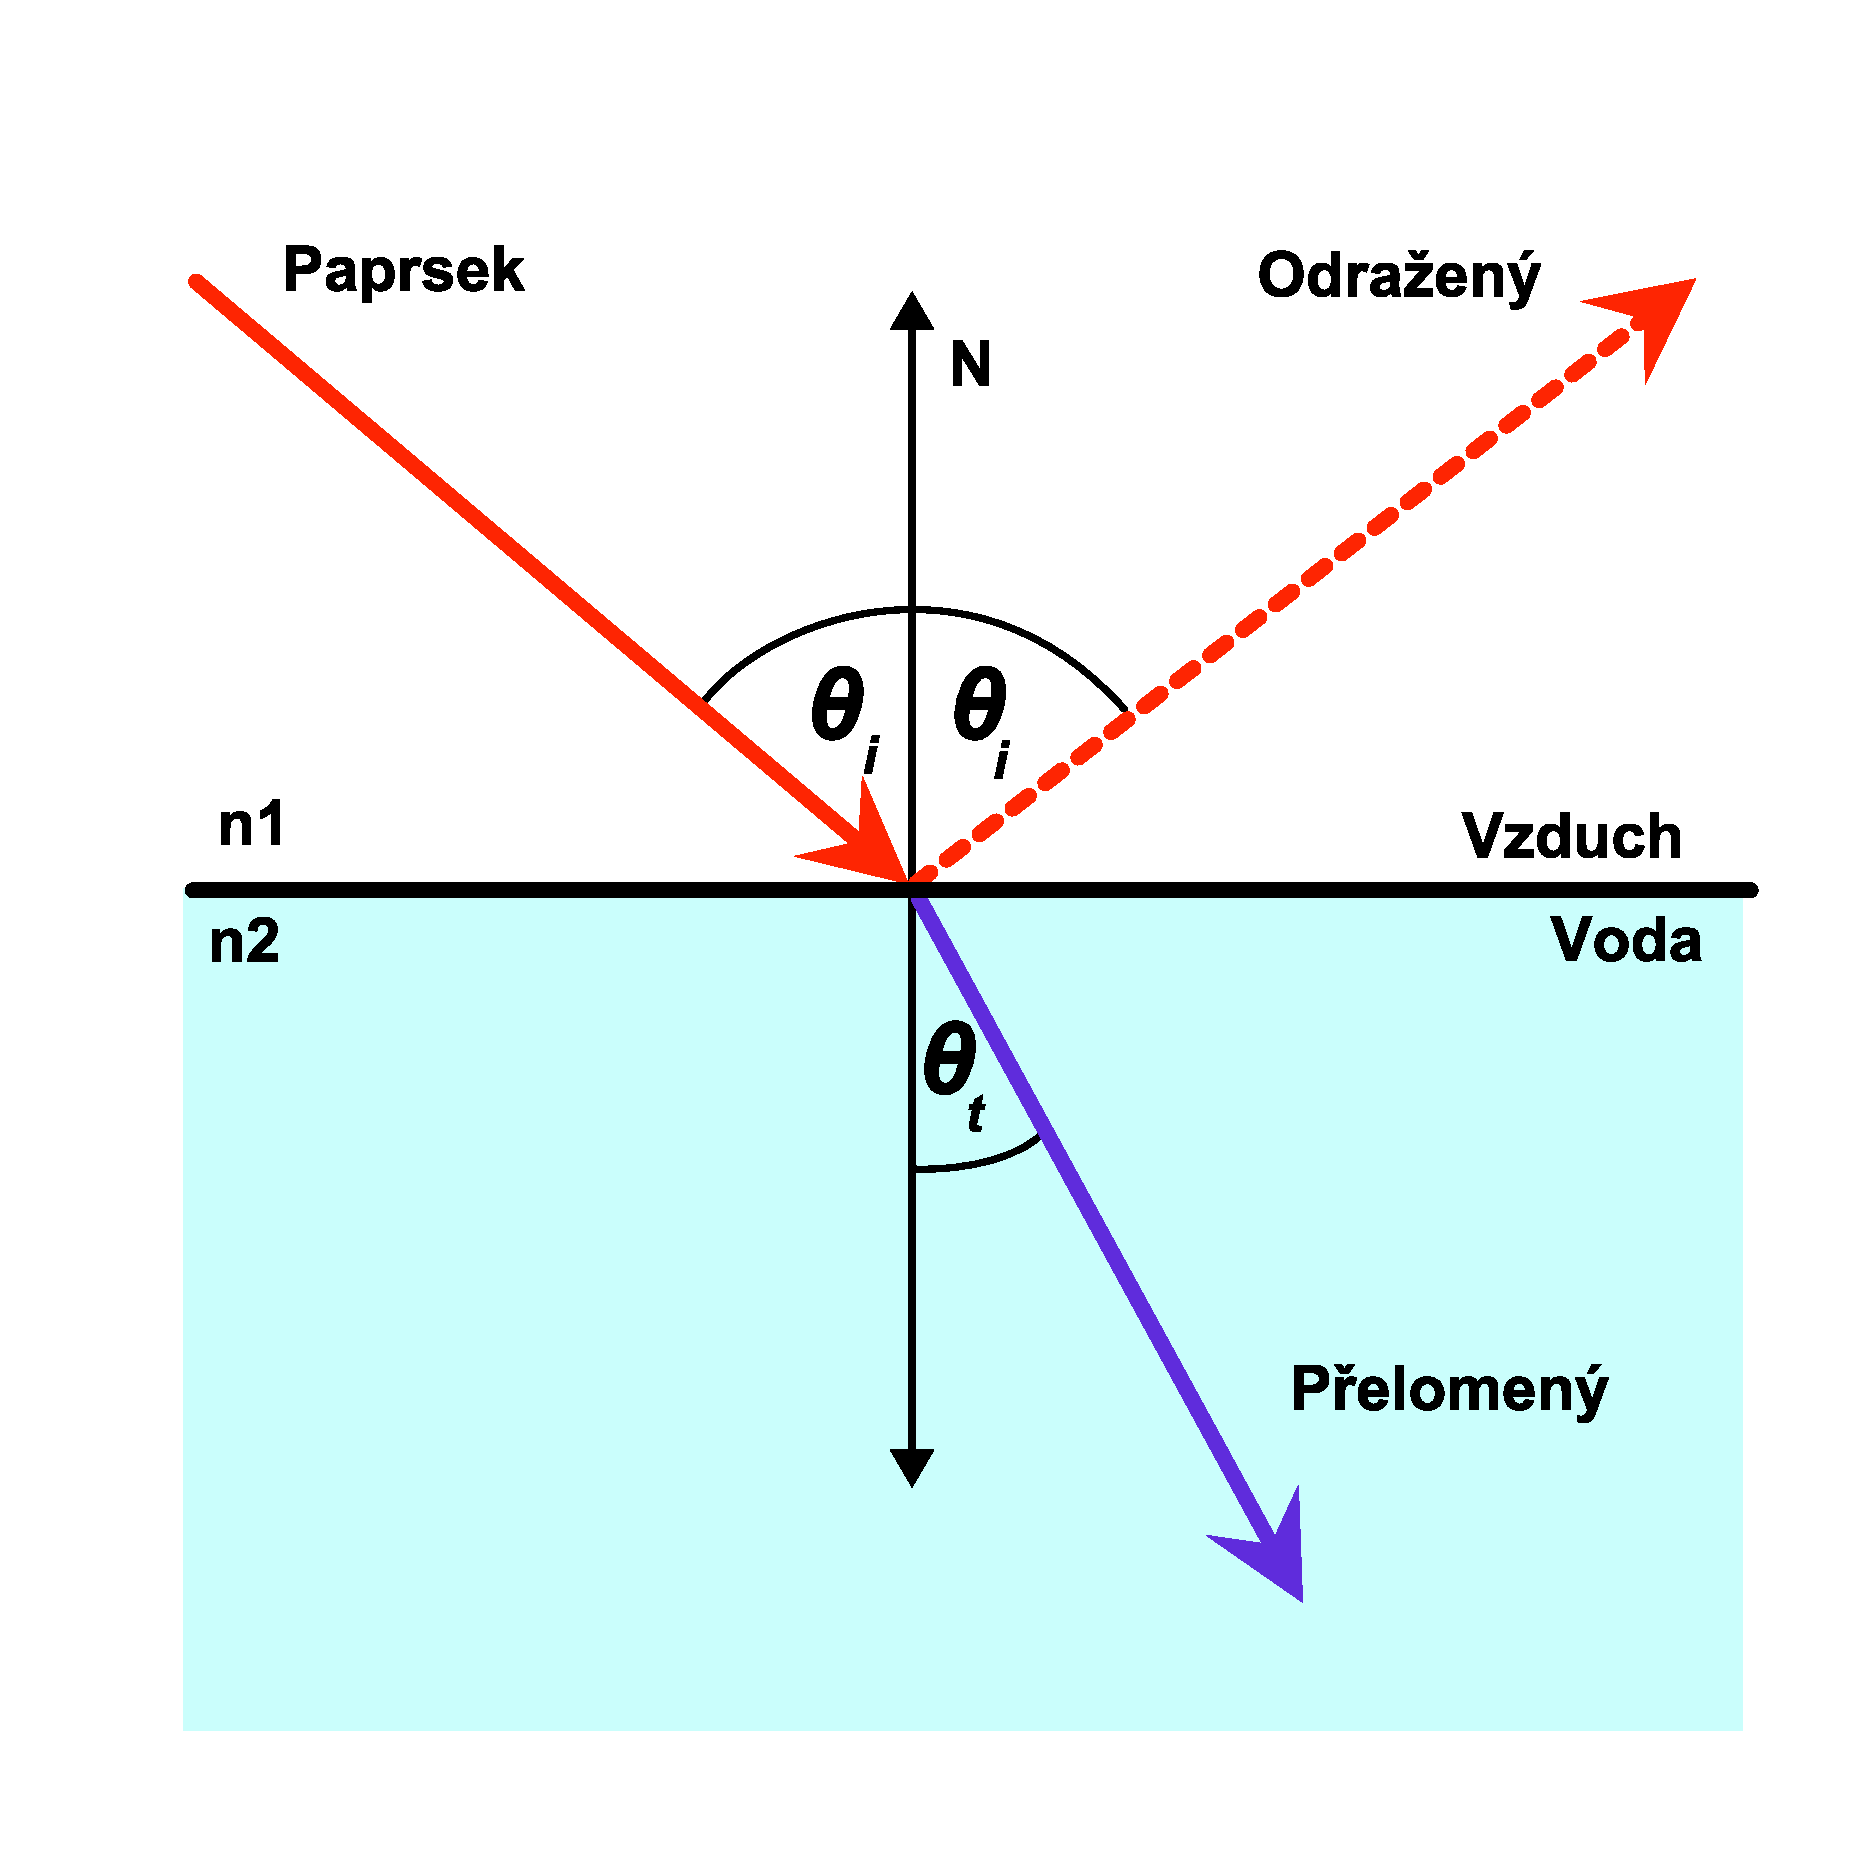
\includegraphics[width=9cm]{obrazky/11}
	\caption{Odrážení světla\cite{3}}
	\label{fig:11}
\end{figure}

\subsubsection{Rychlost přenosu}

Rychlost, se kterou světlo prochází transmisním prostředím, je určena indexem lomu tohoto prostředí. Index lomu prostředí $n$ je poměr rychlosti světla ve vakuu k rychlosti světla v tomto prostředí \cite{3}.

\begin{equation}
n = c / v,
\end{equation}

kde $n$ je index lomu přenosového prostředí, $c$ rychlost světla ve vakuu, a $v$ je rychlost světla v přenosovém prostředí.
Typické hodnoty $n$ pro sklo používané jako optické vlákno jsou mezi 1,45 a 1,55. Čím vyšší je index lomu, tím nižší je rychlost v přenosovém prostředí \cite{3}.

\begin{figure}[ht]
	\centering
	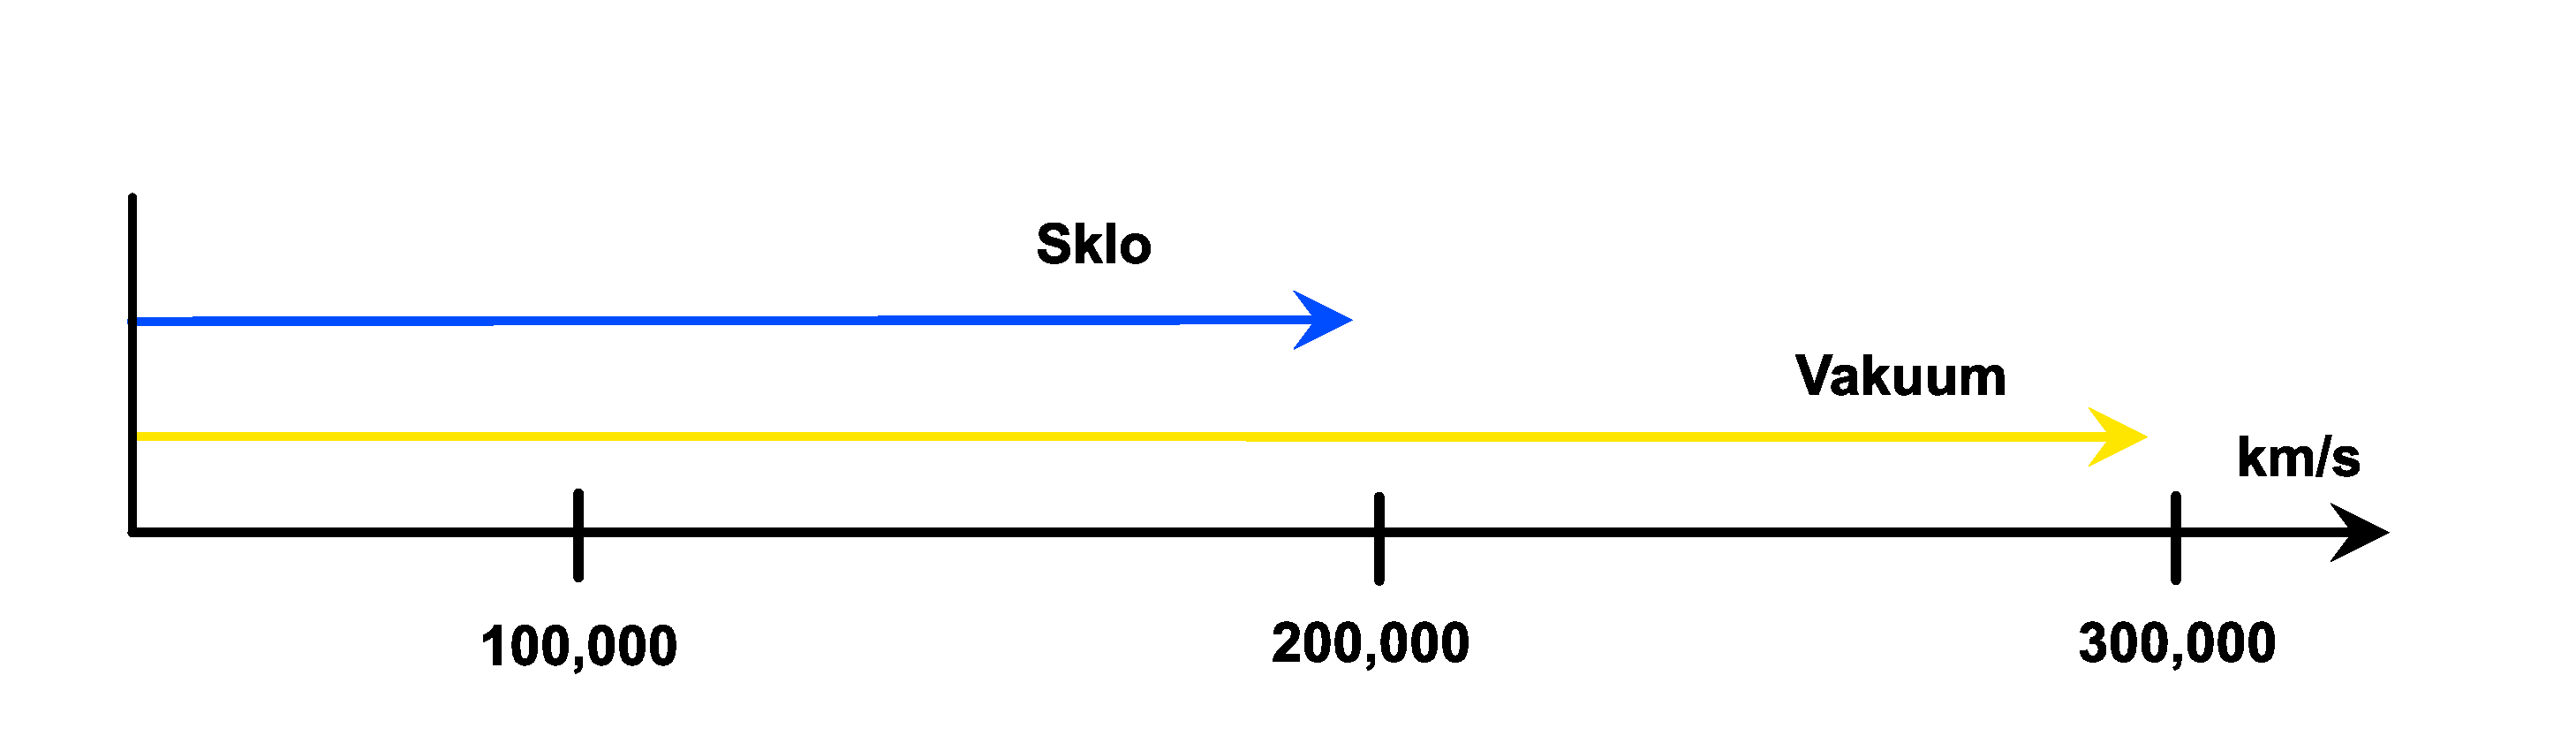
\includegraphics[width=13cm]{obrazky/04}
	\caption{Porovnání rychlosti světla v různých prostředí\cite{3}.}
	\label{fig:04}
\end{figure}

\subsection{Zvuk jako akustické vibrace}

Mechanické vlnění je děj, při němž se kmitání šíří látkovým prostředím. Šíření vln není spojeno s přenosem látky. Vlněním se přenáší energie. Vlnová délka je délka opakujícího se úseku vlny, značíme ji $\lambda$. Frekvence vlny vyjadřuje počet vlnových délek, které vlna urazí za 1~s. Vlnová délka $\lambda$ souvisí s frekvencí vlny $f$ rovnicí, $\lambda = \frac{c}{f}$, kde c je rychlost šíření vlny. Místo frekvence vlny se často používá úhlová frekvence vlny $\omega = 2\pi f$. Fáze popisuje stav vlny v daném místě $\overrightarrow{r}$ čase $t$, v jednorozměrném případě je vyjádřena vztahem $\omega(t - x/c)$ \cite{12}.

\subsubsection{Akustická intenzita}

Střední časová hodnota měrného akustického výkonu za dobu jedné periody je akustická intenzita, $I = \overrightarrow{N}$. Pro rovinnou vlnu získáme akustickou intenzitu: 

\begin{equation}
I = \frac{1}{T}\int_0^T\frac{p^2_{max}}{\rho c}sin^2\omega(t - x/c)dt = \frac{p^2_{ef}}{\rho c},
\end{equation}

kde $p_{ef}$ je efektivní hodnota akustického tlaku definovaná rovnicí

\begin{equation}
p_{ef} = \frac{1}{T}\int_0^Tp^2dt.
\end{equation}

Akustická intenzita pro rovinnou vlnu tedy souvisí s akustickým tlakem rovnicí~\cite{12} 

\begin{equation}
I = \frac{p^2_{ef}}{\rho c}.
\end{equation}

\subsubsection{Šiřění akustických vln} 

V uzavřeném prostoru (v místnosti) dochází k odrazu akustické energie od stěn, stropu a podlahy zpět směrem ke zdroji. To má za následek zvýšení hladiny akustického tlaku v porovnání se stavem, který by vznikl ve volném prostoru. Významnou roli zde hraje pohltivost zvuku povrchů, které ohraničují uzavřený prostor \cite{13}.

Při dopadu zvuku o akustickém výkonu $P_0[W]$ na překážku se část tohoto výkonu $P_r[W]$ odrazí a část $P_a[W]$ pohltí. Pohlcený výkon se pak rozdělí na část výkonu $P_l[W]$, která se ztratí (je odvedena konstrukcí mimo sledované místo nebo se promění v jiný druh energie) a na část $P_t[W]$, která projde stěnou a je vyzářena do vedlejšího prostoru. Lze definovat činitele odrazu vzorec $\rho = P_r/P_0$, činitele pohltivosti $\alpha = P_\alpha/P_0$ a činitele prostupu (průzvučnosti) $\tau = P_t/P_0$. Tito tři činitelé jsou bezrozměrná čísla, která mohou nabývat hodnot od nuly do jedné \cite{13}.

Na obr. \ref{fig:42} je schéma řezu uzavřeným prostorem (místností) se zdrojem zvuku uprostřed. Formou pravoúhlého diagramu je naznačeno rozložení hladin akustického tlaku v prostoru. Na svislé ose diagramu je stupnice hladin akustického tlaku $L[dB]$, na ose vodorovné je vzdálenost $r[m]$ od zdroje zvuku. Jestliže se zvýší celková pohltivost prostoru například obložením stropu místnosti zvuk pohlcujícím obkladem, hladina v poli odražených vln $L1[dB]$ se sníží na hodnotu $L2[dB]$. Zároveň se zvětší dozvuková vzdálenost z hodnoty $r_{k1}[m]$ na hodnotu $r_{k2}[m]$. Z vyobrazení je zřejmé, že zvýšením celkové pohltivosti prostoru nelze snížit hladinu akustického tlaku v bezprostřední blízkosti zdroje, kde se nachází pole přímých vln. Hladinu akustického tlaku $L[dB]$ v poli odražených vln je možno stanovit pomocí vztahu (68). Jeho odvození vychází z vlastností difúzního zvukového pole a respektuje zákon zachování energie. To znamená, že akustický výkon vyzařovaný zdrojem musí být celý pohlcován ohraničujícími povrchy místnosti. Po spuštění zdroje zvuku se hladina akustického tlaku v poli odražených vln ustálí právě na takové hodnotě, která zajistí stav rovnováhy mezi vyzářeným a pohlceným akustickým výkonem \cite{13}.
 
\begin{figure}[ht]
	\centering
	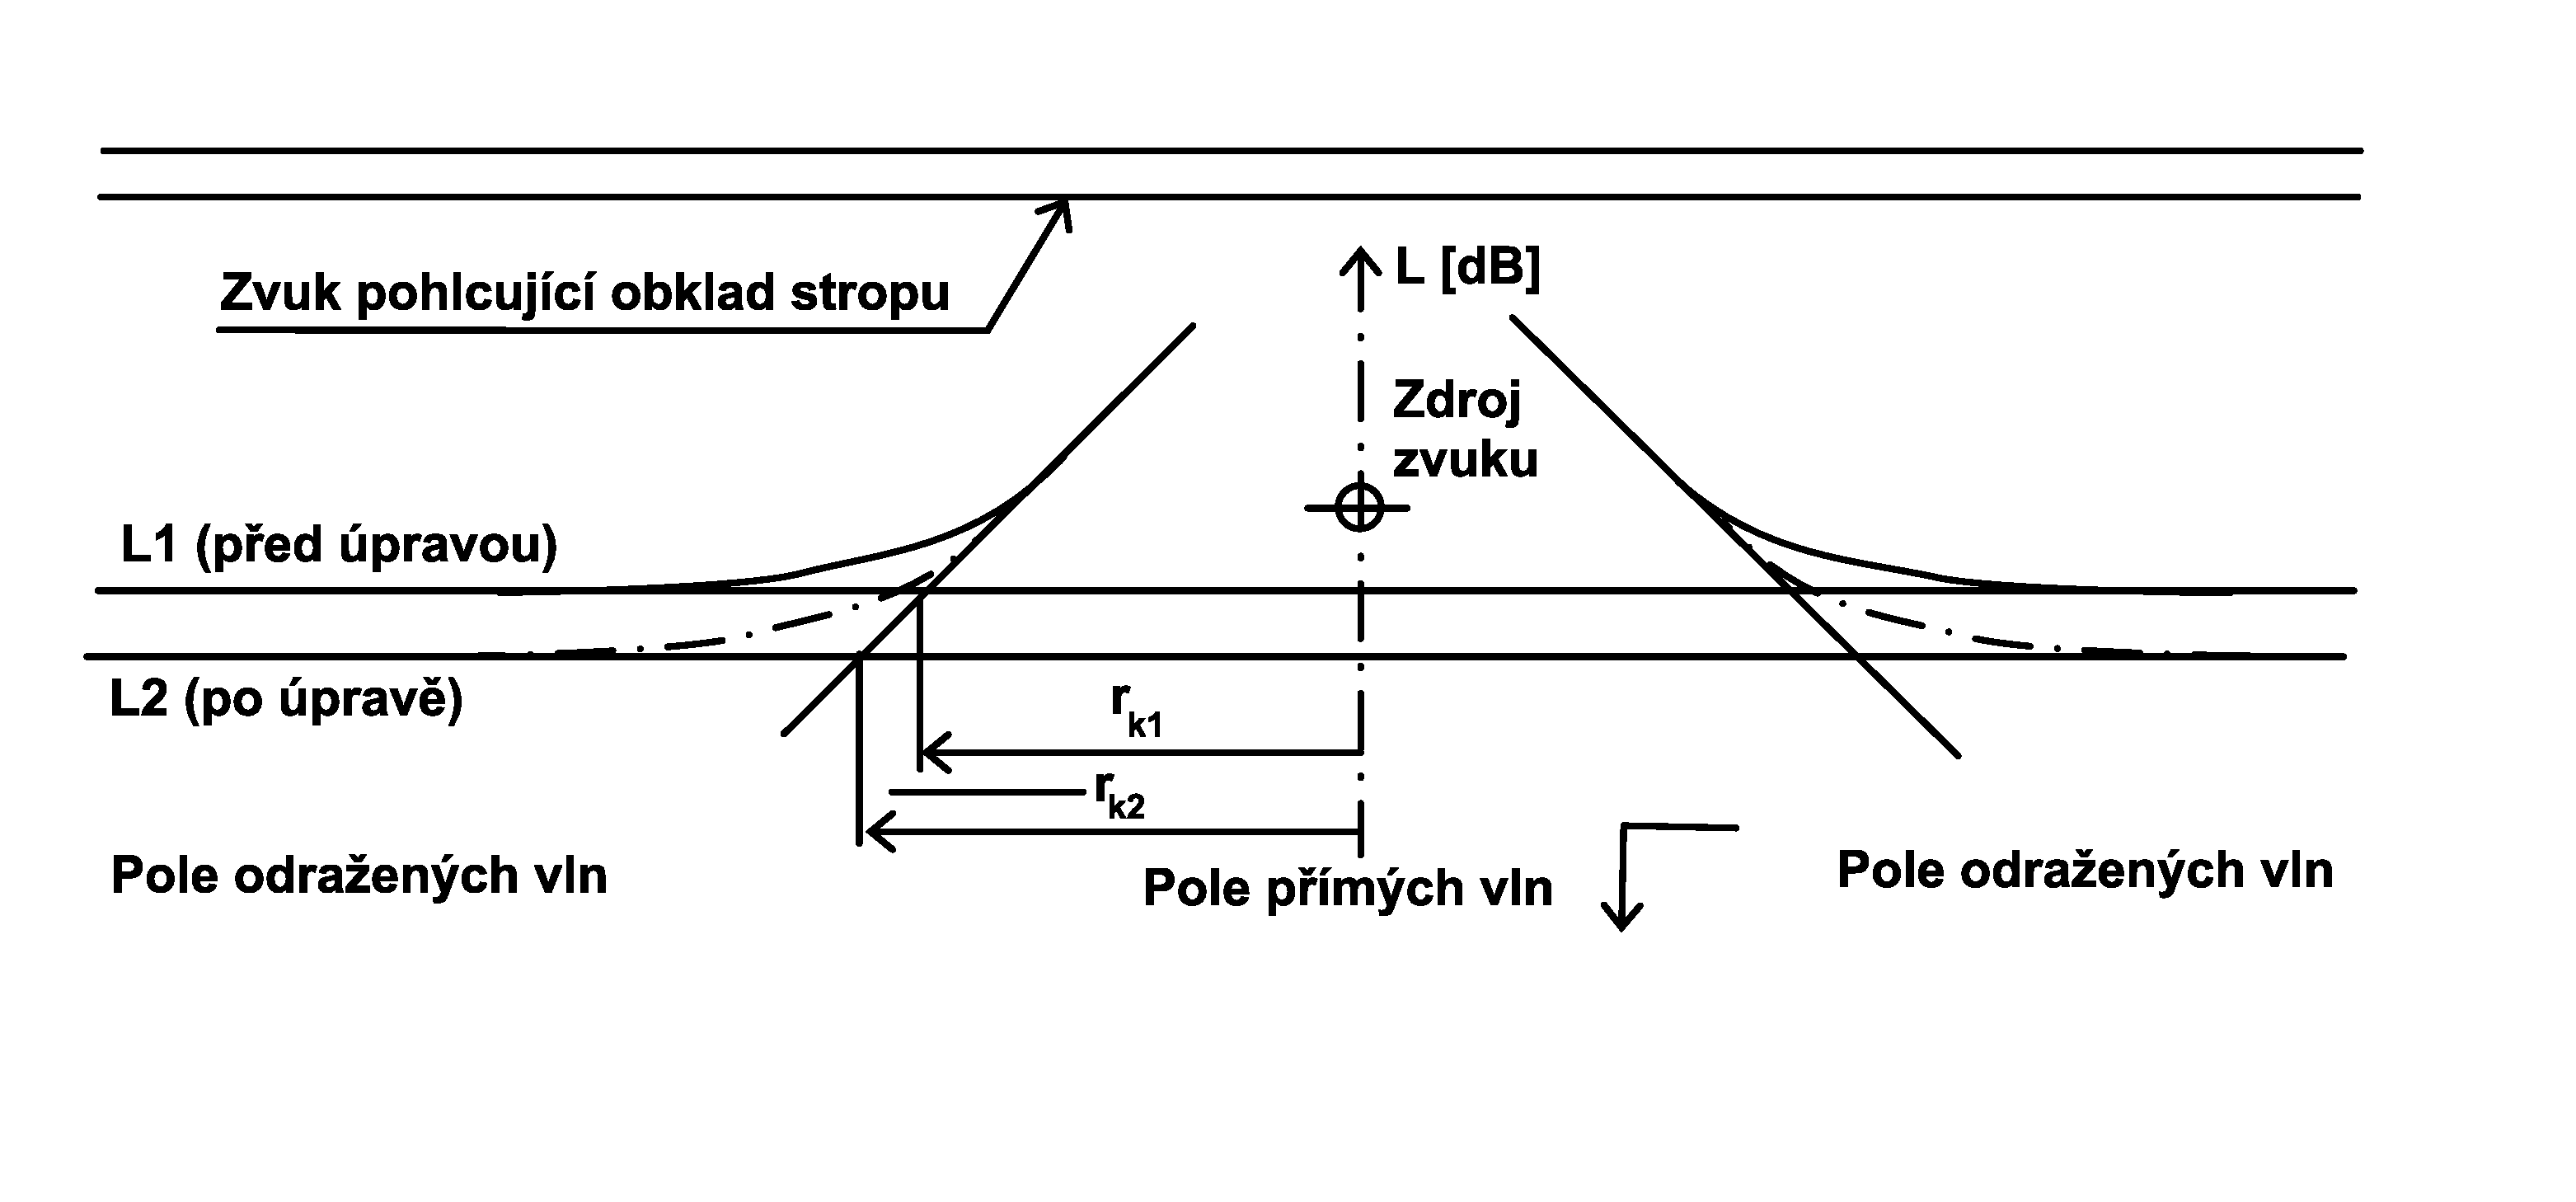
\includegraphics[width=14cm]{obrazky/42}
	\caption{Pole přímých vln a pole odražených vln \cite{13}}
	\label{fig:42}
\end{figure}

\subsection{Interakce akustických vln s optickým vláknem}

Existuje několik možností ovlivnění akustické vlny na laserový paprsek: zavedení akustických kmitů do optického vlákna přes pevné spojení mezi kmitajícím prvkem a kabelem z optických vláken \cite{402} a bezkontaktní vliv akustické vlny na laserový paprsek. V obou případech akustická vlna generuje periodickou kompresi a vzácnou interakci prostředí v jádru, které světelná vlna <<vidí>> jako periodickou změnu indexu lomu. Výsledkem je ekvivalent Braggové mřížky s <<zrnem>> rovná amplitudě vibrací na konci transformátoru a optické vlákno. Rovnice, která ukazuje vztah mezi indexem lomu a délkou optického vlákna \cite{419}:

\begin{equation}
\Delta(\frac{L}{n^2}) = \sum P_{ij}S_{ij} = -\frac{2\Delta n}{n^3},
\end{equation}

kde $P_{ij}$ - faktor foto-elasticity, $S_{ij}$ - složka tenzorné deformaci, $n$ - index lomu, $L$ - délka optického vlákna. 
Fázový posun v optickém vláknu lze dát do následující rovnice \cite{419, 420}:

\begin{equation}
\Delta\phi = \frac{knL(e_3 - n^2)}{2(P_{11}e_1 + P_{12}e_2 + P_{12}e_3)},
\end{equation}

kde $e_1$, $e_2$, $e_3$ představují hlavní elongační faktory, $P_{11}$ a $P_{12}$ jsou faktory foto-elasticity, $k$ je číslo optické vlny.

Periodickou změnu indexu lomu v prostředí během kmitání harmonického napětí lze vyjádřit jako \cite{421}:

\begin{equation}
\Delta n = -\frac{n^3}{2}P_{11}S_0 cos(\Omega t - k_s z),
\end{equation}

kde $S_0$ - maximální amplituda deformace způsobená zvukovou vlnou, $\Omega$ - frekvence akustické vlny, $k_s$ - délka vlnového vektoru (propagační konstanta akustické vlny).
V případě zavedení zvukových kmitů na optické vlákno pevným spojením mezi kmitájícim prvkem a optickým vlákném se vyskytují tyto jevy\cite{406, 407}:

\begin{itemize}

\item fázová modulace způsobená změnami indexu lomu

\item oscilace hrotu optického vlákna

\end{itemize}

\subsubsection{Fotoelastický efekt}

Přítomnost kmenového pole v jakémkoli materiálu vede ke změně optického indexu lomu. Tento vztah je vyjádřen matematicky:

\begin{equation}
\Delta\varepsilon_{ij} = \varepsilon_{ii}\varepsilon_{jj}p_{ijkl}S_{kl},
\end{equation}

kde $\Delta\varepsilon_{ij}$ je změna dielektrického tenzoru, $\varepsilon_{ij}$ a $S_{kl}$ je tenzor napětí. To souvisí pomocí tenzoru tenzoru napětí, $p_{ijkl}$, které jsou uvedeny v tabulce pro různé materiály \cite{421}. Tímto způsobem optický paprsek může být rozptylován podle Snellova zákonu, zatímco on prochází přes pole napětí. Tento jev je znám jako elastooptický efekt.

Tenzové pole může být indukováno množící se akustickou vlnou, která má za následek periodiku modulace dielektrické konstanty frekvencí rovnou frekvenci akustické vlny, $(f_a = \omega_a/2\pi)$. Tato periodická porucha funguje jako pohybující se difrakce a je principem za akusticko-optickými zařízeními \cite{421}.

\section{Optické vlákno v realizaci optických vláknových mikrofonů}

Mikrofon z optických vláken přeměňuje akustické vlny na elektrické signály, které reagují na změny intenzity světla namísto detekování změn kapacitance nebo magnetických polí, na rozdíl od tradičních mikrofonů.
Světlo prochází z laserového zdroje optickým vláknem, které osvětluje povrch reflexní membrány. Zvukové vibrace membrány modulují intenzitu světla odrazeného od membrány v určitém směru. Poté modulované světlo prochází dalším optickým vláknem do fotodetektoru, který transformuje světlo na analogový nebo digitální zvukový signál, připravený pro vysílání nebo nahrávání\cite{5}.

Optické vláknové mikrofony mají vysoký dynamický a frekvenční rozsah a jsou srovnatelné s vysoce přesnými klasickými mikrofony. Optické vláknové mikrofony (OVM) nereagují na účinky elektrického, magnetického, elektrostatického nebo radiačního pole. Proto jsou OVM ideální pro použití v místech, kde je použití tradičních mikrofonů neefektivní nebo nebezpečné (například v plynových turbínách)\cite{5}.
 
OVM jsou spolehlivé, odolné vůči změnám teploty a vlhkosti pracovního prostředí. Vzdálenost mezi laserovým zdrojem mikrofonu a jeho fotodetektorem může dosáhnout několika kilometrů bez jakýchkoliv zesilovačů nebo jiných elektronických zařízení\cite{5}.

\subsection{Princip činnosti optických vláknových mikrofonů}

Optická vlákna, která jsou sloupcová, se skládají z jádrové vrstvy a potahové vrstvy. Systém snímání optických vláken se skládá hlavně ze zdroje světla, snímacích optických vláken, snímací jednotky a systému zpracování signálu. V současné době byly postupně vyvinuty senzory s optickými vlákny s různými typy modulace, včetně typu fáze, typu intenzity, typu vlnové délky a polarizace \cite{337}.

V důsledku působení vnějších zvukových vln se index lomu a průměr jádra fázově modulovaného vlákno-optického senzoru změní, čímž se změní propagační cesta optického signálu ve vlákně a nakonec dojde ke změně fáze. Vzhledem k vysoké frekvenci světla však nelze pomocí stávající detekční technologie fázovou změnu světelné vlny detekovat přímo. Ale pokud jde o změnu intenzity světla, lze ji snadno zjistit. Proto se fázová změna obvykle v experimentu mění na změnu intenzity světla a poté se akustický signál získá pomoci demodulační technologií \cite{337}. 
Předpokládá se, že amplitudy dvou paprsků jsou $E_1$, respektive $E_2$. Pokud je fáze jednoho světla modulována vnějšími akustickými poruchami, je druhé světlo izolováno od vnějších poruch, takže není ovlivněno. Intenzita interferenčního světla pak může být vyjádřena jako:

\begin{equation}
E^2 = E_1 + E_2 + 2E_1E_2cos(\delta\phi + \phi_0),
\end{equation}

kde $\phi_0$ je počáteční fázový rozdíl mezi dvěma koherentními paprsky. $\delta\phi$ je fázový rozdíl způsobený fázovou modulací, který přímo odpovídá intenzitě interferenčního světla. Detekcí intenzity interferenčního signálu lze stanovit fázovou změnu mezi dvěma paprsky světla a změřené fyzikální parametry lze demodulovat. Technologie interferometrického snímání přitahovala rozsáhlou pozornost a výzkum díky svým širokým vyhlídkám na použití v oblasti  akustického měření. V současné době jsou fázově modulované akustické snímače optických vláken založeny hlavně na třech principech interference: Mach-Zehnderová interference (MZI), Michelsonová interference (MI) a Sagnacková interference (SI) \cite{338}.

\subsubsection{Machová-Zehnderová konfigurace}

První práce v oblasti optického akustického snímání byla provedená J.A. Bucarem \cite{21}. Jeho detekční metoda byla postavená na optickém vláknovém Machovém-Zehnderovém interferometru (MZI). Působení akustické vlny na jednu paži vláknového interferometru ukázalo, že interakce akustických vln s vlákném vede ke změně délky optické dráhy. Proto charakteristiku akustické vlny lze odvodit z pozorovaní změn v intenzitě výstupu interferometru. Tento interferometr pracoval se zvukovými frekvencemi 40 kHz -- 400 kHz bez významné změny citlivosti. Vlákno MZI bylo použito v mnoha sestavách pro další studium schopností optických vláknových akustických senzorech a zejména vytváření hydrofonů z optických vláken \cite{211}. Další důležité práce s využitím nastavení vláknového MZI byla demonstrována v roce 2007 \cite{212}, kde byla konfigurace založena na pracovní cestě Hockera při zvyšování citlivosti pomocí potahování vlákna kompozitními strukturami s nízkou hodnotou modulu pružnosti . Ukázalo se, že přidáním piezoaktivního polymerního povlaku k vláknu bylo možné zvýšit citlivost ke akustické vlně\cite{213}. 

Základní princip obecného Machova-Zehnderova optického vláknového interferometru je znázorněn na obrázku \ref{fig:32}. Koherentní světlo emitované laserovým zdrojem je optickým vazebním členem 1×2 rozděleno na dva samostatné paprsky. Po průchodu vazebním členem jsou paprsky přenášeny dvěma cestami, které jsou pojmenované jako měřicí rameno a referenční rameno \cite{212}. 

\begin{figure}[ht]
	\centering
	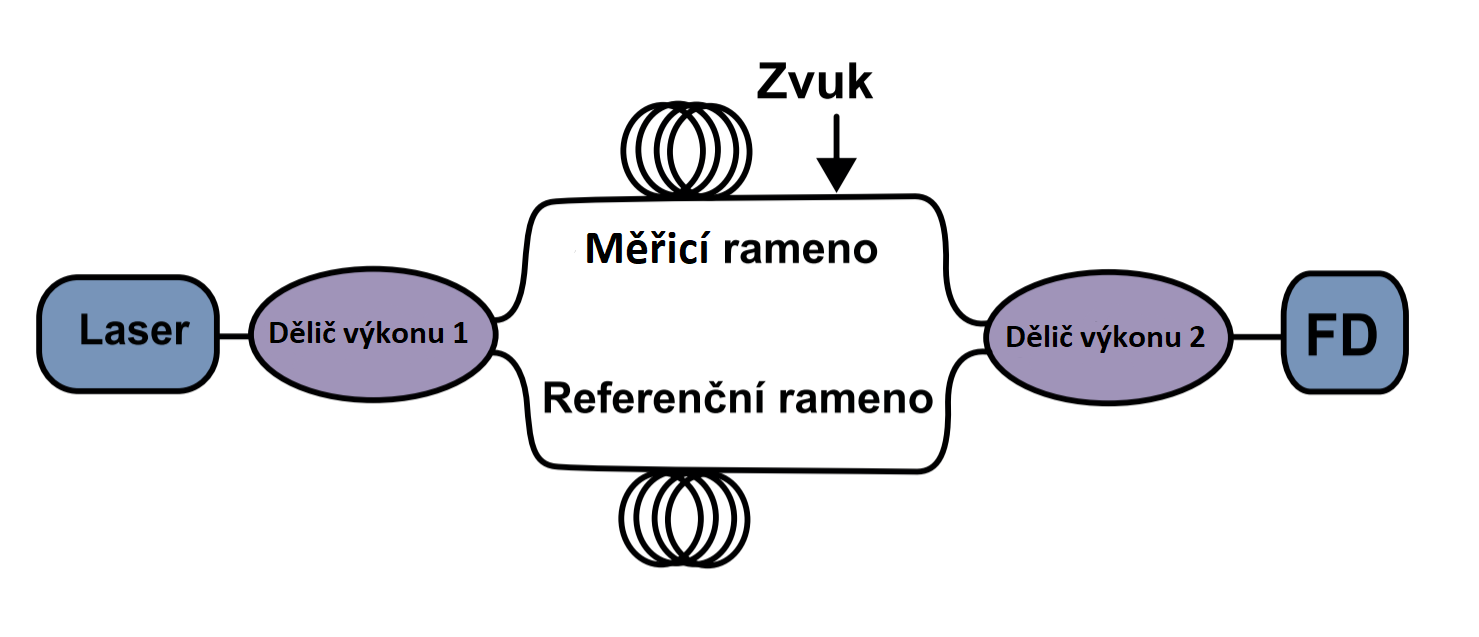
\includegraphics[width=12cm]{obrazky/32}
	\caption{Struktura Machové-Zehnderové interference \cite{501}.}
	\label{fig:32}
\end{figure}

Když na měřicí rameno působí vnější akustický tlak, velikost vlákna snímacího ramene je natažená nebo zkrácená a index lomu snímacího ramene se mění, což je způsobené fázovou modulací optického signálu. Nicméně, referenční rameno je izolováno nějakou látkou tak, že není ovlivněno vnějším akustickým tlakem. Modulované světlo a referenční světlo je spojeno spojovacím zařízením 2×1 a pak se vzájemně ovlivňují. Interferenční signál je přijímaný fotodetektorem, a pak je akustický signál získaný následným procesem demodulace signálu. Podle zásady interference to naznačuje, že když dva paprsky se stejnou frekvencí a stejným směrem vibrací se navzájem interferuje, interferenční intenzitu světla lze vyjádřit jako \cite{212}:

\begin{equation}
I = I_1 + I_2 + 2\sqrt{I_1I_2}cos(\delta\phi), 
\end{equation}

kde $I_1$ a $I_2$ jsou počáteční intenzity obou paprsků a $\delta\phi$ je počáteční fázový rozdíl mezi těmito dvěma paprsky.
V tuto chvíli lze fázový rozdíl $\delta\phi$ dvou paprsků, které vzájemně interferují, považovat za součet následujících tří faktorů: počáteční fázový rozdíl $\phi_1$ v důsledku asymetrie samotných dvou optických drah, fázový rozdíl $\phi_s$ v důsledku vnějšího tlaku a fázový rozdíl $\phi_{\epsilon}$  vyplývající ze změny délky vlákna způsobené napětím, které lze vyjádřit jako \cite{212}:

\begin{equation}
\delta\phi = \phi_0 + \phi_ + \phi_{\epsilon}.
\end{equation}

Počáteční fázový rozdíl $\phi_0$ je konstantní hodnota, takže změna intenzity světla detekovaná fotodetektorem souvisí pouze se změnami výše uvedených fázových rozdílů $\phi_1$ a $\phi_{\epsilon}$. Je tedy možné vypočítat odpovídající změnu fázového rozdílu $\delta\phi$ dvou paprsků po dosažení změny intenzity. Akustické vibrace, působící na signální rameno, mohou být získány analýzou fázového rozdílu.
Tento jediný Machův-Zehnderův interferometr dokáže snadno detekovat akustické signály. Následně, za účelem dalšího umístění akustického zdroje, se postupně zkoumá distribuovaný systém snímání s duální strukturou Macha-Zehndera (DAS)\cite{240}, jak je znázorněno na obrázku \ref{fig:31}.

\begin{figure}[ht]
	\centering
	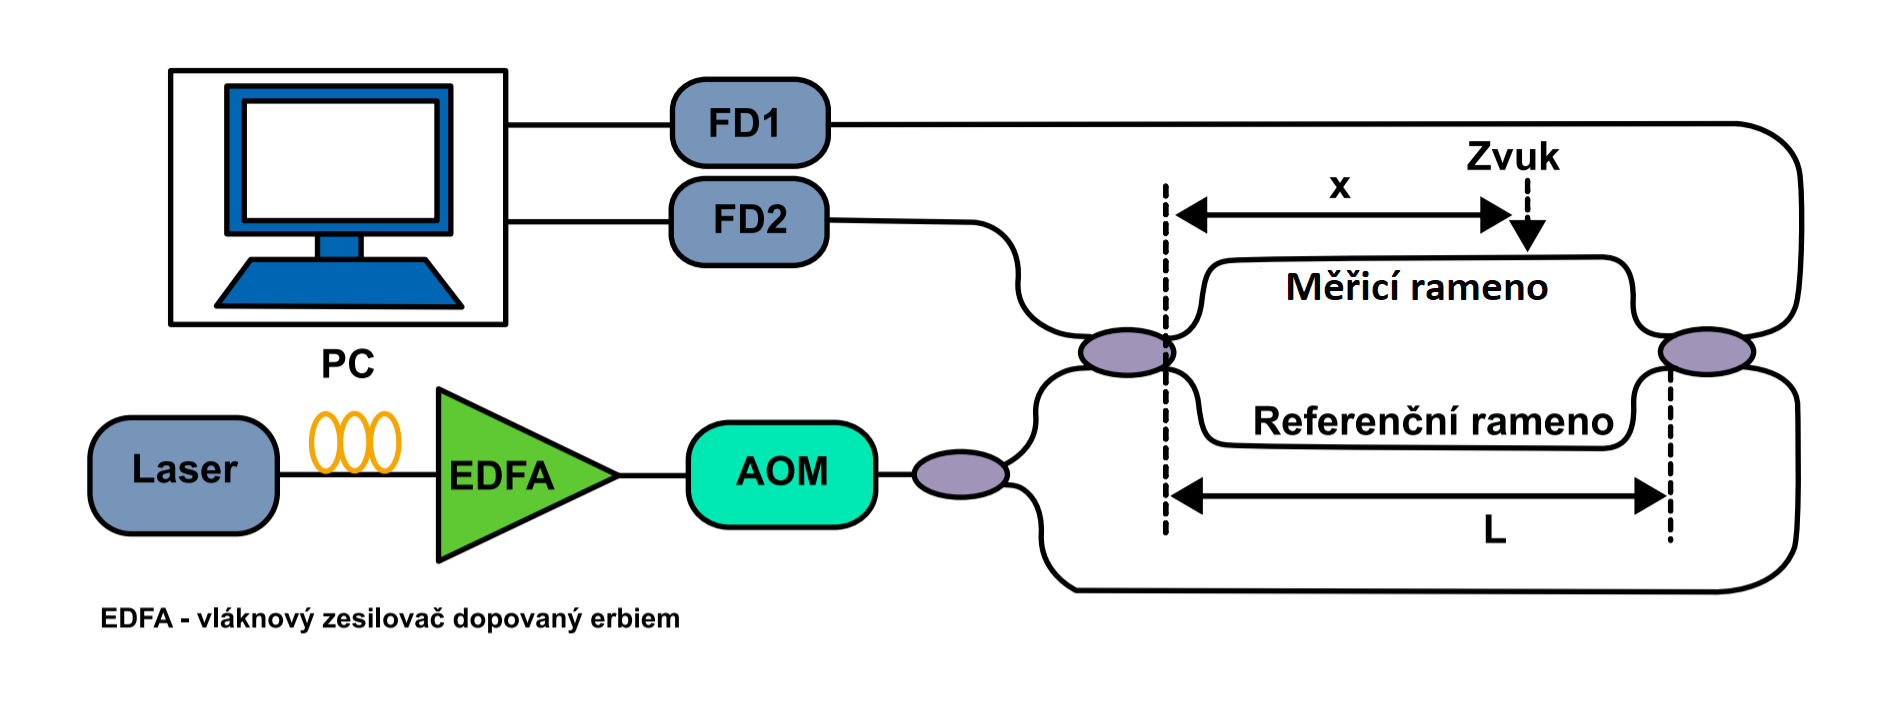
\includegraphics[width=16cm]{obrazky/31}
	\caption{System DAS s duální strukturou Mach-Zehndera \cite{501}.}
	\label{fig:31}
\end{figure}

Po zesílení a modulaci se světlo, emitované laserem, rozdělí na paprsky ve směru hodinových ručiček a proti směru hodinových ručiček vazebním členem 1×2. Dva světelné signály procházejí vazebním členem 2 a vazebním členem 3, interferují na konci cest a poté jsou přijímány fotodetektory. Na obrázku \ref{fig:31}, pokud je délka referenčního ramene nastavena na 1 a vzdálenost mezi vazebním členem 2 a akustickým zdrojem je nastavena na $x$, časové zpoždění obou světelných drah může být vyjádřeno jako \cite{241}:

\begin{equation}
d = \frac{2l - x}{c/n} - \frac{x}{c/n} = \frac{2n}{c}(l - x),
\end{equation}

kde $c$ představuje rychlost světla ve vakuu a $n$ představuje index lomu jádra vlákna. Odhadnutím časového zpoždění je možné realizovat umístění akustického zdroje.
Distribuované akustické senzory založené na interferometru Mach-Zehndera se vyznačují nízkými náklady, jednoduchou strukturou a dlouhým dosahem snímání \cite{241}.

\subsubsection{Michelsonova konfigurace}

Optické vláknové Michelsonovy interferometry se také používájí pro akustickou detekcí \cite{215, 216}. Michelsonova konfigurace sestává z optického vláknového vazebního členu, kde se používají dvě výstupní ramena jako referenční a senzorové cesty. Na konci každé paže existuje reflexní struktura (např. zrcadlo nebo FBG) pro odeslání dvou signálů zpět do detektoru. Lze si představit Michelsonovo nastavení (viz obr.\ref{fig:33}) jako polovina Mach-Zehndera, který provádí svou činnost velmi podobným principem. Ačkoli v tomto případě, místo toho segmentu vlákna, který je detektorem, je možné, že se jedná o odraznou strukturu akustického převodníku, zodpovědného za optický rozdíl v cestě. Michelsonská konfigurace je pravděpodobně nejméně používaná konfigurace pro vláknové optické akustické snímání.

Snímací schéma optické dráhy založené na Michelsonovém optickém vláknovém interferometru je znázorněna na obrázku \ref{fig:33}.

\begin{figure}[ht]
	\centering
	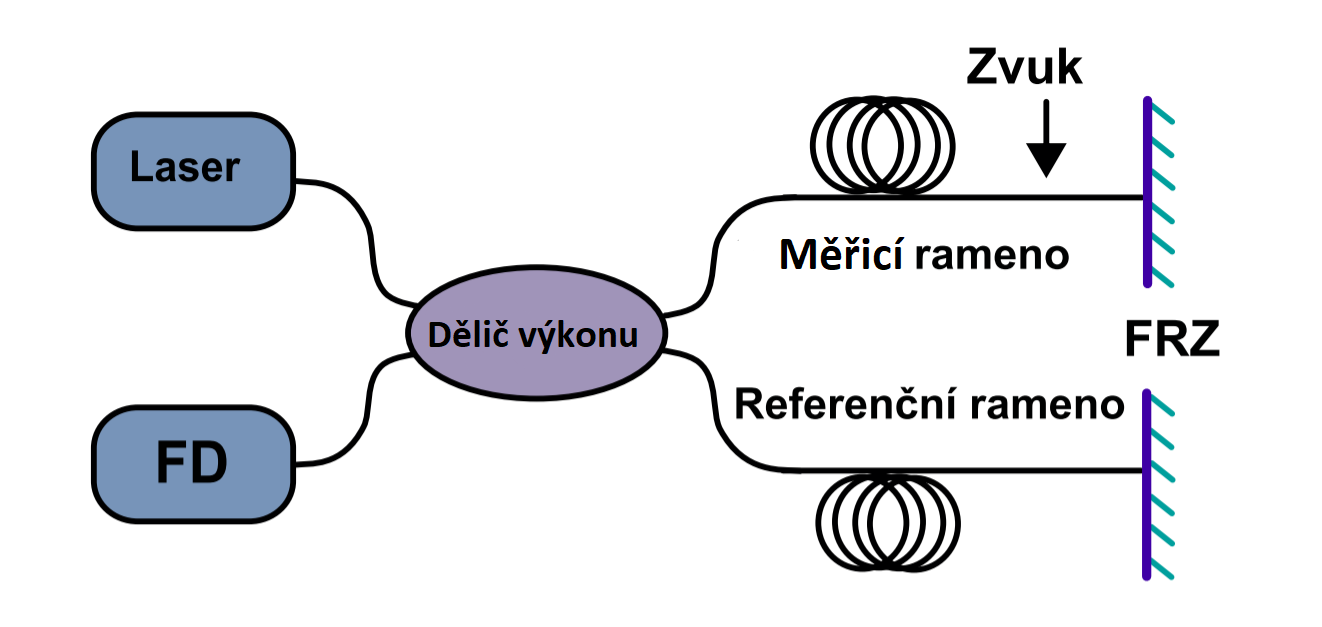
\includegraphics[width=10cm]{obrazky/33}
	\caption{Strukturální schéma Michelsonova interferometru \cite{501}.}
	\label{fig:33}
\end{figure}

Mezi nimi je reflexivní konec odkazu a snímací vlákna jsou důležitou součástí optického vláknového interferometru. Poté, co prošel děličem výkonu, signál emitovaný světelným zdrojem je rozdělen na dva kanály, jeden přes referenční vláknové rameno, druhý přes měřicí rameno, které je působené vnějším zvukem. Při dosažení zrcadla se dva paprsky světla odráží zpět do děliče výkonu a vzájemně se ovlivňují. Interferenční světlo nese zvukové informace. Po detekování fotoelektrickými detektory se předpokládá změna intenzity světla kteké se nakonec převede na elektrický signál. Poté může se demodulovat zvukový signál. Intenzita světla přijímaného fotodetektorem lze vyjádřit jako\cite{215}:

\begin{equation}
P = P_0(1 + cos(\delta\phi)),
\end{equation}

kde $\delta\phi$ je fázový rozdíl způsobený akustickým tlakem mezi referenčním světlem a signálním světlem. Ve srovnání s interferometrem Mach-Zehndera, struktura Michelsonova interferometru používá méně vazebných vláken a snižuje optickou ztrátu. Jeho hlavní nevýhodou však je, že interferenční signál, odražený do fotodetektoru, se bude také odrážet na laserovém zdroji, který bude mít negativní dopad na normální provoz laseru a formování šumu. Proto, aby se eliminoval tento druh šumu, je nutné zvýšit kvalitu použití optického izolátoru \cite{216}.

Michelsonův optický vláknový systém má jasný princip, jednoduchou strukturu a vysokou teoretickou hodnotu. Mnoho vědců zkoušelo různé demodulační algoritmy pro další optimalizaci výkonu systému.

\subsubsection{Sagnacova konfigurace}

Sagnacův optický vláknový interferometr je také jedna z nejvíce prozkoumaných konfigurací pro optické akustické snímání \cite{26, 217}. Tento interferometr byl široce používány při výrobě optických vláknových hydrofonových systémů pro akustické detekce. Obrázek \ref{fig:34} (a) představuje typickou konfiguraci Sagnacova optického vláknového interferometru. Konečná variace amplitudy je funkce fázové modulace hydrofonu a výsledkem akustické modulace frekvence s časovým zpožděním smyčky. To se liší od MZI senzorů, kde konečná amplituda je funkce pouze modulace hydrofonové fáze. Smyčka bude mít správnou frekvenci, což je nejnižší frekvence, ve které se dosáhne maximální citlivosti. Tato frekvence je určena délkou zpoždění smyčky. Prostředek ke zkrácení délky vlákna použitého v každém senzoru je vyžadován, aby bylo možné používat Sagnacovy senzory ve velkém měřítku. Poprve byla Sagnacova konfigurace demonstrováná v roce 1999 \cite{218}. 

Princip funkce je následující: dopadající světlo je rozděleno na dvě části  ve směru hodinových ručiček (CW) a proti směru hodinových ručiček (CCW) a šíři podél smyčky optického vlákna vazebním členem 50:50. Po celém cyklu zasahují do děliče výkonu. Když vnější zvuk působí na optické vlákno, index lomu af fáze se měni. Po demodulace fotodetektorem (PD) se tyto změny transformují na změny intenzity světla \cite{217}.

\begin{figure}[ht]
	\centering
	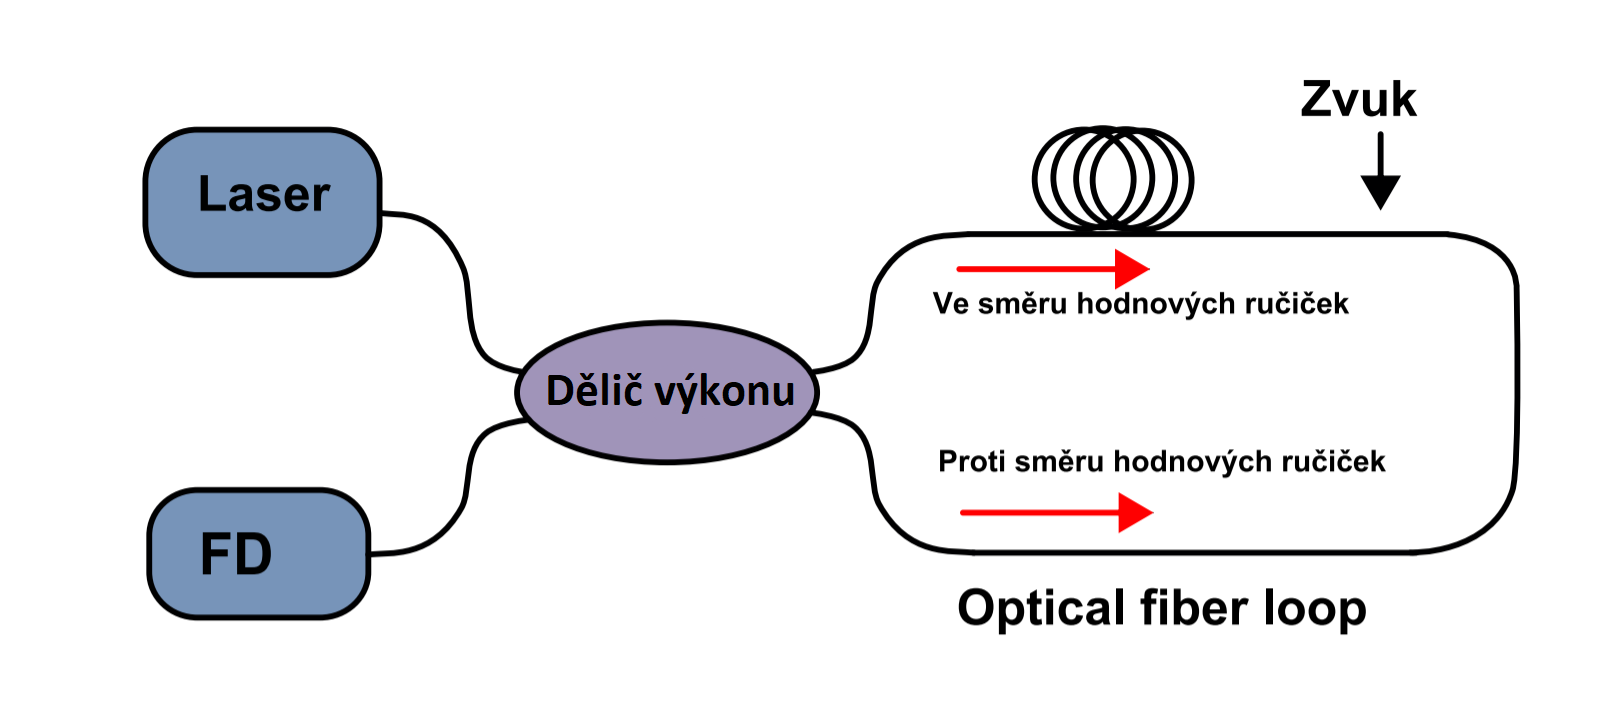
\includegraphics[width=14cm]{obrazky/34}
	\caption{Princip děje Sagnacůva interferometru \cite{501}.}
	\label{fig:34}
\end{figure}

Když paprsek světla prochází optickým vláknem o délce $l$, fázové zpoždění $\Delta\Phi$ vyvolané akustickým signálem je následující:

\begin{equation}
\delta\Phi = \beta(\Delta l) + l(\Delta\beta) = \beta(\Delta l) + l\frac{\delta\beta}{\delta n} + l\frac{\delta\beta}{\delta d}.
\end{equation}

Ve vzorci $d$ označuje průměr jádra snímacího vlákna a $\beta$ je propagační konstanta světelné vlny v optických vláknech, $\beta = nk_0$, kde $n$ je index lomu jádra, $k_0$ je počet vln světla ve vakuu, $k_0 = 2\pi/lambda_0$ je vlnová délka světla ve vakuu.
První neznámá ve vzorci představuje fázový rozdíl $\Delta\phi_1$ (Strainův efekt) způsobený změnou délky snímacího vlákna, druhou položkou je fázový rozdíl $\Delta\phi_n$ (elastický světelný efekt) způsobený změnou indexu lomu snímaného vlákna, a třetí položkou je fázový rozdíl (Poissonův efekt) způsobený změnou průměru jádra snímacího vlákna, které lze obecně zanedbat kvůli jeho malé relativné hodnotě \cite{217}.

\begin{equation}
\delta\Phi = \beta(\Delta l) + l\frac{\delta\beta}{\delta n} = \Delta\phi + \Delta\phi_n.
\end{equation}

Světlo ve směru a proti směru hodinových ručiček interferuje s vazebním členem a výstupní interferenční signál nese fázovou interferenci způsobenou akustickým signálem. Vztah mezi vnějším akustickým signálem a intenzitou výstupního světla lze vyjádřit takto \cite{217}:

\begin{equation}
I = I_0(1 + cos(\Delta\phi)) = 4I_0cos^2(\frac{\Delta\phi}{2}).
\end{equation}

\subsubsection{Fabryová-Pérotová konfigurace}

Zájem o interferometry Fabry-Pérota (FPI) pro vytvoření akustických senzorů z optických vláken rostl s časem, a v dnešní době se důkladně zkoumají \cite{27}. Tento interferometr získal význam v roce 2006 v oblasti akustického snímání s jeho demonstraci v roce 1991 \cite{219}. Vnější dutina Fabry-Pérota (FP) sestávalá ze vzduchové mezery mezi single-mode vláknem a multimode vláknem, vše uvnitř dutého vlákna, jak je znázorněno na obr. \ref{fig:24} (a). Změny vzduchové mezery kvůli použitému napětí modifikovaly vlastnosti FP dutiny. 
Změny v dutině lze odvodit pomocí analýzy změny vlnové délky odražených vln, a proto napětí vznikající z akustické vlny lze určit. Existuje mnoho demonstrací vnějších FPI pro tlakové a akustické snímání používající optická vlákna \cite{220}.

\begin{figure}[ht]
	\centering
	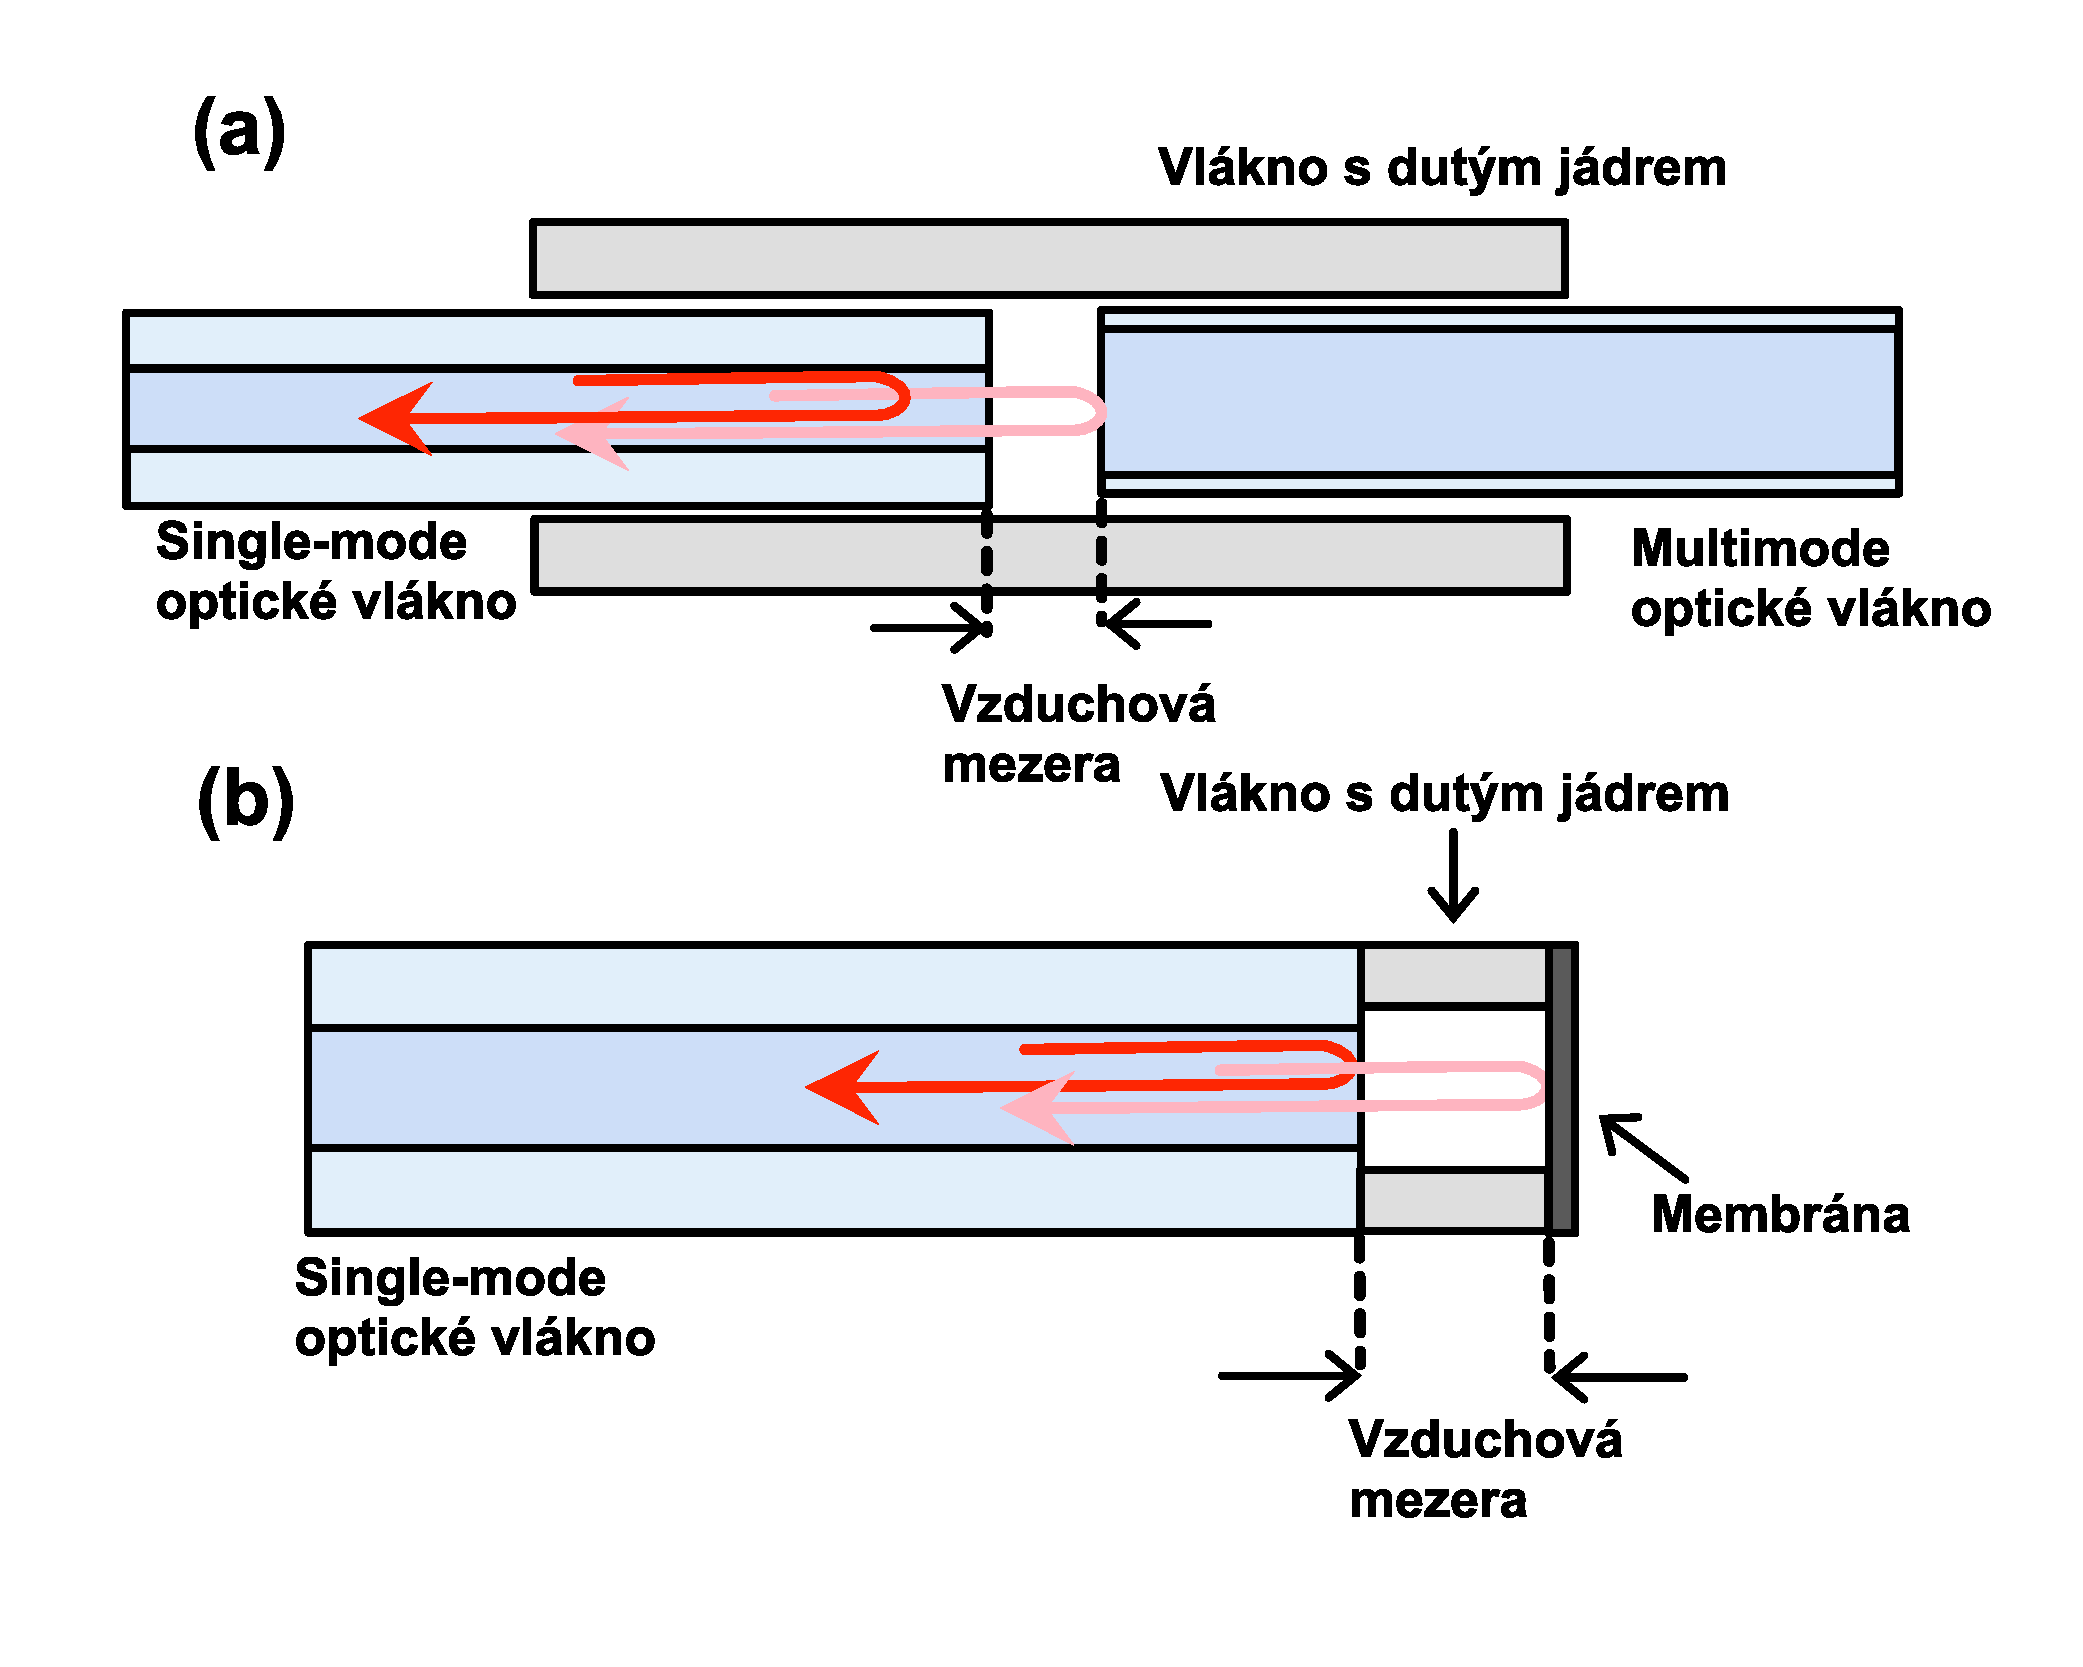
\includegraphics[width=12cm]{obrazky/24}
	\caption{Vnější interferometr Fabry-Pérota: a) vzduchová mezera (b) dutina na bázi bránice \cite{500}}
	\label{fig:24}
\end{figure}

K interferenci dochází v důsledku více superpozic odrazených i přenášených paprsků na dvou rovnoběžných plochách. Poté, co světlo projde dutinou F-P, foto detektor (PD) přijíme interferenční signál a převede jej. Pokud akustický tlak působí na membránu, změna fáze $\Delta\Phi$ optické vlny lze jednoduše vyjádřit jako:

\begin{equation}
\Delta\Phi =  \frac{4\pi n\Delta L}{\lambda_0},
\end{equation}

kde $n$ představuje index lomu prostředí plnicího dutinu, $\lambda_0$ je optická vlnová délka ve vakuu, $\Delta L$ označuje vychýlení bránice a lze vyjádřit jako:

\begin{equation}
\Delta L =  \frac{P\delta^4(1-\nu^2)}{4.2Eh^3},
\end{equation}

kde $P$ je okolní tlak související s tlakem dutiny, $\delta$ představuje délku poloviny okraje, $\nu$ je Poissonův poměr materiálu bránice, $E$ odkazuje na modul Younga a $h$ je tloušťka membrány.
V FPI senzoru jeho citlivost $S$ při pokojové teplotě vyjádřeno jako:

\begin{equation}
S =  \frac{3\delta^4(1-\nu^2)}{16Eh^3},
\end{equation}

V akustickém snímání, založeném na FPI systému, může být citlivost detekce zlepšena ze dvou aspekty: tloušťka membrány a délka poloviny okraje. Membránový materiál je tedy pro snímače F-P kuriozní. Obvykle materiály membrány dutiny Fabry-Perota obsahují hlavně mikro křemíkový film, kovový film \cite{220}.

\subsubsection{Braggovy vláknové mřížky} %todo

Optické FBG (Fiber Bragg gratings) byly poprvé představeny Hillem v~roce 1978~\cite{230}. Jak je znázorněno na obr. \ref{fig:25}, FBG je periodická mikrostruktura tištěná pomocí změn indexu lomu jádra vlákna. Struktura bude odrážet pouze specifickou vlnovou délku, což závisí na pravidelných rozestupech FBG. Analýzou posunů v odražené vlnové délce lze určit odchylku mezer. Mnoho senzorů může být postaveno na principu FBG. Nejčastěji používané jsou tenzometrické a teplotní senzory založené na FBG \cite{230}. \\

\begin{figure}[ht]
	\centering
	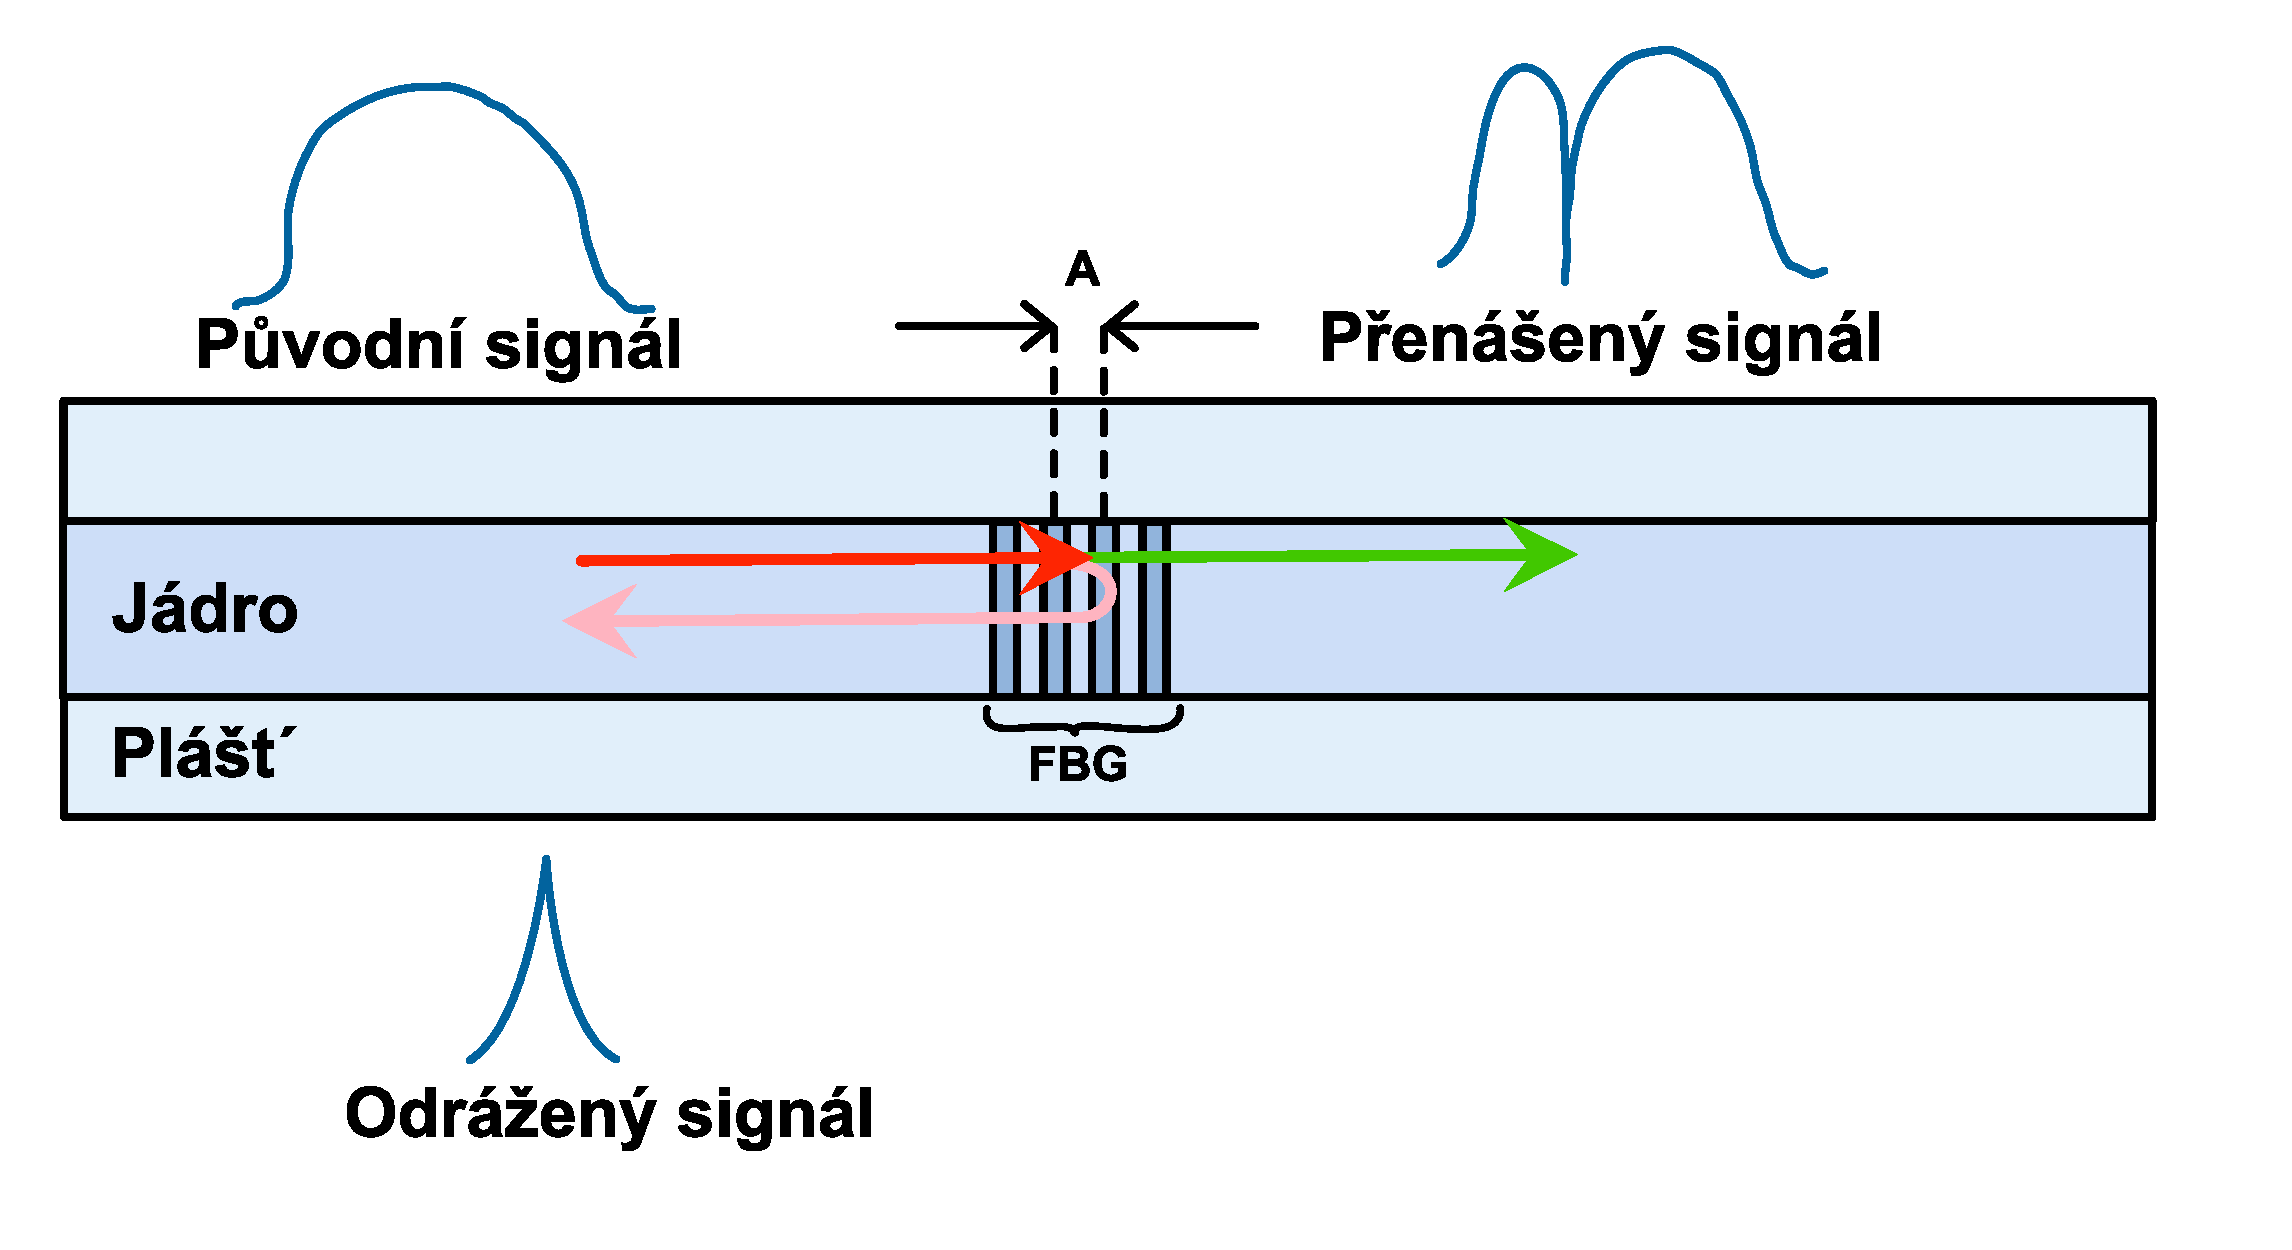
\includegraphics[width=12cm]{obrazky/25}
	\caption{Princip činnosti optického senzoru založeného na FBG (odražená Braggova vlnová délka $\lambda_B$ souvisí s periodou $\Lambda$ FBG prostřednictvím $\lambda_B = 2n_e\Lambda$, kde $n_e$ je efektivní index lomu struktury) \cite{500}.}
	\label{fig:25}
\end{figure}

Braggovy vláknová mřížka (FBG) je optické pasivní zařízení, což je senzor vytvořený periodickou modulací axiálního indexu lomu jádra optického vlákna. Má tyto výhody: dobrá stabilita, vysoká citlivost a snadné spojení s jinými optickýmy vlákny.
Když akustický signál působí na optické vlákno, efektivní index lomu a další parametry optického vlákna se změní. Když dopadající světlo vstoupí na FBG, vztah mezi centrální vlnovou délkou odrazu $\lambda_B$, efektivním indexem lomu $n_{eff}$ a období strouhání $\Lambda$ je následující \cite{323}:

\begin{equation}
\lambda_B = 2n_{eff} \Lambda.
\end{equation}

Když je FBG působená akustickým signálem, efektivní index lomu a doba strouhání se změní, což vede k posunu centrální vlnové délky odraženého světla. Změny posunu způsobené akustickými signály mohou být vypočteny jako \cite{324}:

\begin{equation}
\Delta\lambda_B = 2n_{eff} \Delta\Lambda + 2\Lambda\Delta 2n_{eff}.
\end{equation}

Intenzita výstupního světla, která je teoreticky poměrná akustickému signálu, může být získána pomocí demodulací Braggovy vlnové délky.

Akustické senzory FBG lze také použít v akustických hydrofonech, nedestruktivním posuzování, biomedicínském snímání a sledování strukturálního zdraví \cite{326}. Systém má takové výhody, jako jsou vysoká rychlost a vysoká přesnost.

\subsection{Optické vláknové mikrofony v komerci}

Rakouská společnost Xarion Laser Acoustics GmbH, založená v roce 2012 jako spin-out společnost Vídeňskou technologickou univerzitou a společností Knowles Corporation, přináší optický mikrofon bez membrány s bezprecedentním rozlišením zvuku.
<<Pro nedestruktivní testování můžeme pracovat jednostranně s emitorem zvuku na straně mikrofonu. Skenováním povrchu napříč 2D rovinou můžeme identifikovat vnitřní strukturální výchozí hodnoty, které poskytují různé zvukové vzorce,>> vysvětlil CEO\cite{7}.

\begin{figure}[ht]
	\centering
	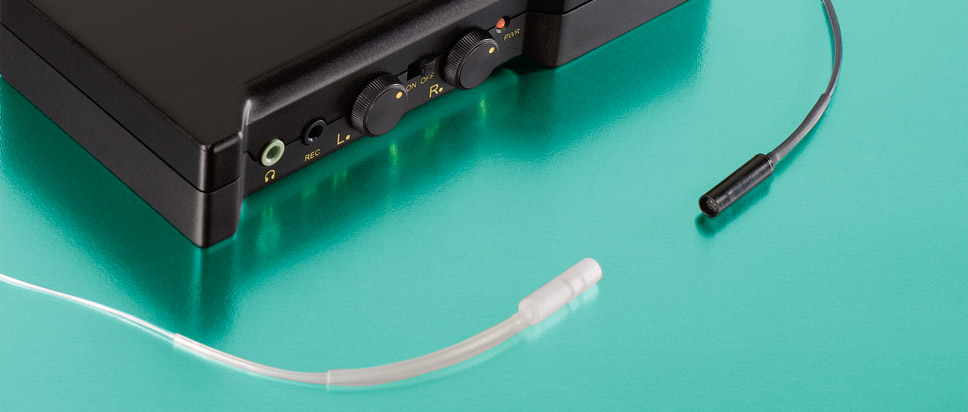
\includegraphics[width=13cm]{obrazky/08}
	\caption{Komerční optický vláknový mikrofon \cite{502}}
	\label{fig:08}
\end{figure}

<<Protože náš optický mikrofon má velmi dobrou fázovou odezvu, je vhodnější pro směrový záznam zvuku než tradiční mikrofony. Pomocí pole 3 až 7 mikrofonů bychom mohli pomocí algoritmů pro vytváření paprsků můžeme poslouchat známé místo a vyhnout se okolním hlukům o 360°>>, tvrdí Fischer.\cite{7}.

\subsubsection{Miniaturní optické vláknové mikrofony}

Běžné mikrofony jsou velké a nejsou vhodné do prostředí s omezeným nebo těžko přístupným prostorem. Kromě toho může přítomnost objemného mikrofonu narušit akustické pole a způsobit chyby měření. Proto už existují ultra-miniaturní, vysoce citlivé a širokopásmové optické mikrofony s celkovou velikostí srovnatelnou s průměrem vlákna (125~μm). Klíčovou součástí mikrofonu je ultratenká (100~nm) kovová fólie připojená k Fabry-Perotově dutině na konci vlákna. Následující obrázky ukazují schéma a obrázek mikrofonu a mikrofonního systému\cite{8}.

\begin{figure}[ht]
	\centering
	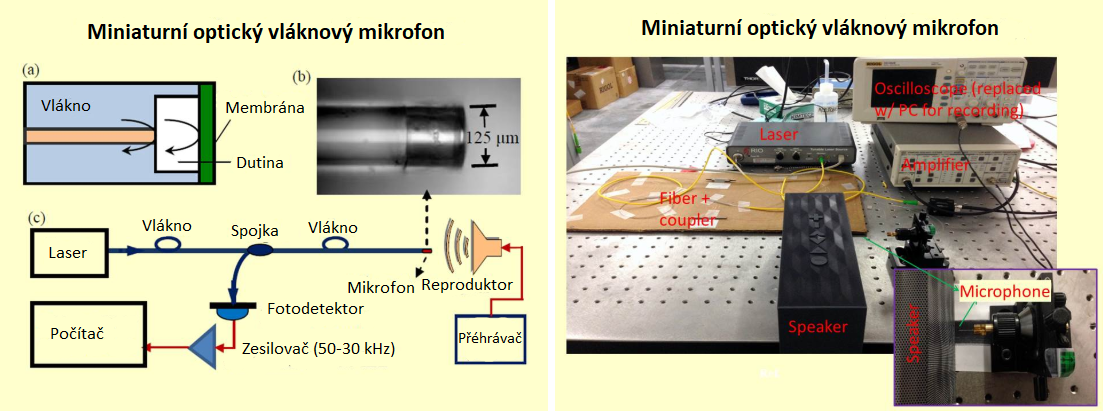
\includegraphics[width=15cm]{obrazky/16}
	\caption{Schéma miniaturního mikrofonu a jeho vzhled\cite{8}}
	\label{fig:16}
\end{figure}

\subsection{Výhody oproti obyčejným mikrofonům}

Tyto mikrofony se snadno schovají a dobře fungují, když jsou zapojené do již existujících sítí optických vláken. Dále je třeba poznamenat, že optické jednovláknové komunikační kanály jsou imunní vůči jakémukoli rušení EMI/RF, takže je lze považovat za absolutně bezpečné a nezjistitelné.

Oproti obyčejným klasickým mikrofonům optické vláknové mají řadu výhod:

\begin{itemize}

	\item OVM maji velkou delku přenosu bez doplňujícího zařízení (může pracovat i 10 km od mikrofonu do elektronické jednotky bez zesilovače)\cite{9}

	\item jsou méně ovlivněny elektromagnetickým zářením
	
	\item tezce odhalitelné
	
	\item jsou citlivější, nez obycejné microfony
	
	\item jsou odolnější vůči vodě
	
	\item mikrofony nevyvolávájí žádné elektromagnetické záření (ani na úkor kapsle, kde je předzesilovač obvykle umístěn v jiných typech mikrofonů, ani na úkor kabelů)\cite{9}
	
	\item můžou dosáhnout mnohem menší velikosti, než klasické mikrofony
	
	\item můžou pracovat v silných magnetických, elektrických nebo rádiových polích
	
	\item frekvence zvuku: 5 Hz až 15 kHz se speciální filtrací mezi 20 Hz a 3 kHz\cite{9}
	
\end{itemize}

